\documentclass{ximera}
\graphicspath{  %% When looking for images,
{./}            %% look here first,
{./pictures/}   %% then look for a pictures folder,
{../pictures/}  %% which may be a directory up.
{../../pictures/}  %% which may be a directory up.
{../../../pictures/}  %% which may be a directory up.
{../../../../pictures/}  %% which may be a directory up.
}

\usepackage{listings}
\usepackage{circuitikz}
\usepackage{xcolor}
\usepackage{amsmath,amsthm}
\usepackage{subcaption}
\usepackage{graphicx}
\usepackage{tikz}
\usepackage{tikz-3dplot}
\usepackage{amsfonts}
\usepackage{mdframed} % For framing content
\usepackage{tikz-cd}

  \renewcommand{\vector}[1]{\left\langle #1\right\rangle}
  \newcommand{\arrowvec}[1]{{\overset{\rightharpoonup}{#1}}}
  \newcommand{\ro}{\texttt{R}}%% row operation
  \newcommand{\dotp}{\bullet}%% dot product
  \renewcommand{\l}{\ell}
  \let\defaultAnswerFormat\answerFormatBoxed
  \usetikzlibrary{calc,bending}
  \tikzset{>=stealth}
  




%make a maroon color
\definecolor{maroon}{RGB}{128,0,0}
%make a dark blue color
\definecolor{darkblue}{RGB}{0,0,139}
%define the color fourier0 to be the maroon color
\definecolor{fourier0}{RGB}{128,0,0}
%define the color fourier1 to be the dark blue color
\definecolor{fourier1}{RGB}{0,0,139}
%define the color fourier 1t to be the light blue color
\definecolor{fourier1t}{RGB}{173,216,230}
%define the color fourier2 to be the dark green color
\definecolor{fourier2}{RGB}{0,100,0}
%define teh color fourier2t to be the light green color
\definecolor{fourier2t}{RGB}{144,238,144}
%define the color fourier3 to be the dark purple color
\definecolor{fourier3}{RGB}{128,0,128}
%define the color fourier3t to be the light purple color
\definecolor{fourier3t}{RGB}{221,160,221}
%define the color fourier0t to be the red color
\definecolor{fourier0t}{RGB}{255,0,0}
%define the color fourier4 to be the orange color
\definecolor{fourier4}{RGB}{255,165,0}
%define the color fourier4t to be the darker orange color
\definecolor{fourier4t}{RGB}{255,215,0}
%define the color fourier5 to be the yellow color
\definecolor{fourier5}{RGB}{255,255,0}
%define the color fourier5t to be the darker yellow color
\definecolor{fourier5t}{RGB}{255,255,100}
%define the color fourier6 to be the green color
\definecolor{fourier6}{RGB}{0,128,0}
%define the color fourier6t to be the darker green color
\definecolor{fourier6t}{RGB}{0,255,0}

%New commands for this doc for errors in copying
\newcommand{\eigenvar}{\lambda}
%\newcommand{\vect}[1]{\mathbf{#1}}
\renewcommand{\th}{^{\text{th}}}
\newcommand{\st}{^{\text{st}}}
\newcommand{\nd}{^{\text{nd}}}
\newcommand{\rd}{^{\text{rd}}}
\newcommand{\paren}[1]{\left(#1\right)}
\newcommand{\abs}[1]{\left|#1\right|}
\newcommand{\R}{\mathbb{R}}
\newcommand{\C}{\mathbb{C}}
\newcommand{\Hilb}{\mathbb{H}}
\newcommand{\qq}[1]{\text{#1}}
\newcommand{\Z}{\mathbb{Z}}
\newcommand{\N}{\mathbb{N}}
\newcommand{\q}[1]{\text{``#1''}}
%\newcommand{\mat}[1]{\begin{bmatrix}#1\end{bmatrix}}
\newcommand{\rref}{\text{reduced row echelon form}}
\newcommand{\ef}{\text{echelon form}}
\newcommand{\ohm}{\Omega}
\newcommand{\volt}{\text{V}}
\newcommand{\amp}{\text{A}}
\newcommand{\Seq}{\textbf{Seq}}
\newcommand{\Poly}{\textbf{P}}
\renewcommand{\quad}{\text{    }}
\newcommand{\roweq}{\simeq}
\newcommand{\rowop}{\simeq}
\newcommand{\rowswap}{\leftrightarrow}
\newcommand{\Mat}{\textbf{M}}
\newcommand{\Func}{\textbf{Func}}
\newcommand{\Hw}{\textbf{Hamming weight}}
\newcommand{\Hd}{\textbf{Hamming distance}}
\newcommand{\rank}{\text{rank}}
\newcommand{\longvect}[1]{\overrightarrow{#1}}
% Define the circled command
\newcommand{\circled}[1]{%
  \tikz[baseline=(char.base)]{
    \node[shape=circle,draw,inner sep=2pt,red,fill=red!20,text=black] (char) {#1};}%
}

% Define custom command \strikeh that just puts red text on the 2nd argument
\newcommand{\strikeh}[2]{\textcolor{red}{#2}}

% Define custom command \strikev that just puts red text on the 2nd argument
\newcommand{\strikev}[2]{\textcolor{red}{#2}}

%more new commands for this doc for errors in copying
\newcommand{\SI}{\text{SI}}
\newcommand{\kg}{\text{kg}}
\newcommand{\m}{\text{m}}
\newcommand{\s}{\text{s}}
\newcommand{\norm}[1]{\left\|#1\right\|}
\newcommand{\col}{\text{col}}
\newcommand{\sspan}{\text{span}}
\newcommand{\proj}{\text{proj}}
\newcommand{\set}[1]{\left\{#1\right\}}
\newcommand{\degC}{^\circ\text{C}}
\newcommand{\centroid}[1]{\overline{#1}}
\newcommand{\dotprod}{\boldsymbol{\cdot}}
%\newcommand{\coord}[1]{\begin{bmatrix}#1\end{bmatrix}}
\newcommand{\iprod}[1]{\langle #1 \rangle}
\newcommand{\adjoint}{^{*}}
\newcommand{\conjugate}[1]{\overline{#1}}
\newcommand{\eigenvarA}{\lambda}
\newcommand{\eigenvarB}{\mu}
\newcommand{\orth}{\perp}
\newcommand{\bigbracket}[1]{\left[#1\right]}
\newcommand{\textiff}{\text{ if and only if }}
\newcommand{\adj}{\text{adj}}
\newcommand{\ijth}{\emph{ij}^\text{th}}
\newcommand{\minor}[2]{M_{#2}}
\newcommand{\cofactor}{\text{C}}
\newcommand{\shift}{\textbf{shift}}
\newcommand{\startmat}[1]{
  \left[\begin{array}{#1}
}
\newcommand{\stopmat}{\end{array}\right]}
%a command to give a name to explorations and hints and theorems
\newcommand{\name}[1]{\begin{centering}\textbf{#1}\end{centering}}
\newcommand{\vect}[1]{\vec{#1}}
\newcommand{\dfn}[1]{\textbf{#1}}
\newcommand{\transpose}{\mathsf{T}}
\newcommand{\mtlb}[2][black]{\texttt{\textcolor{#1}{#2}}}
\newcommand{\RR}{\mathbb{R}} % Real numbers
\newcommand{\id}{\text{id}}

\author{Zack Reed}
\title{Matrices Transform Vectors}

\begin{document}

\begin{abstract}
In this activity, we will explore the most important interpretation of matrices: as linear transformations. All applications and methods for matrices can be motivated by this interpretation.
\end{abstract}
\maketitle

\begin{exploration}\name{Matrices Transform Vectors}

    Let's begin by looking at a plot of many vectors in the plane. This is a very simple example where collections of vectors give human-interpretable data. In this case, the vectors all form the outline of a smiley face, as seen in the figure below:

    \begin{center}
        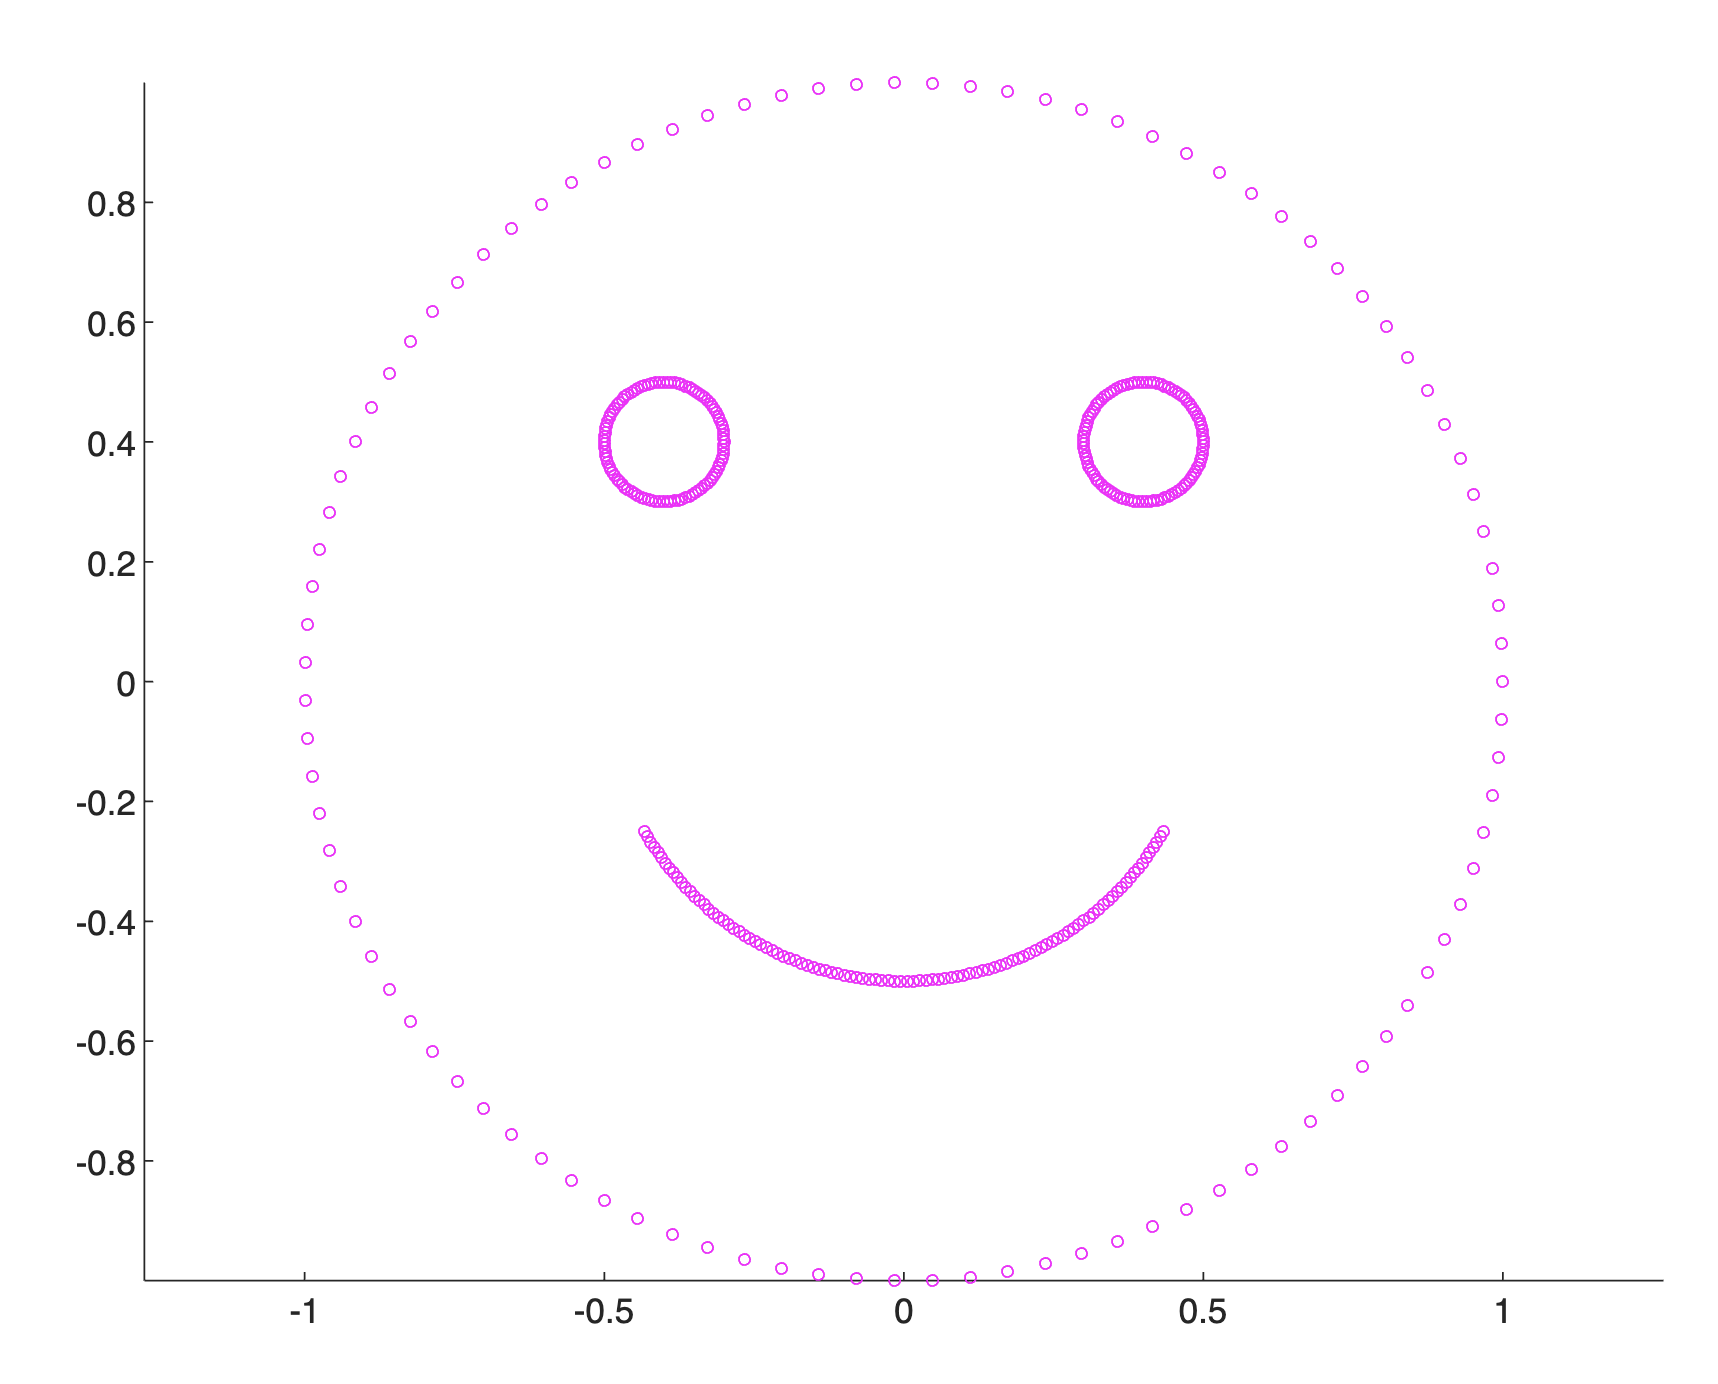
\includegraphics[width=0.5\textwidth]{smiley1.png}
    \end{center}

    \begin{remark}

        Different from other depictions of images in this course, in this case the smiley face is made from vectors in space, whereas in the context of matrices images such as smileyfaces are represented by pixel values within a matrix.

        Recall that we can represent vectors by points or arrows. In this case we want to use points, as arrows can get crowded in plots such as the following, depicting the same smiley face:

        \begin{center}
            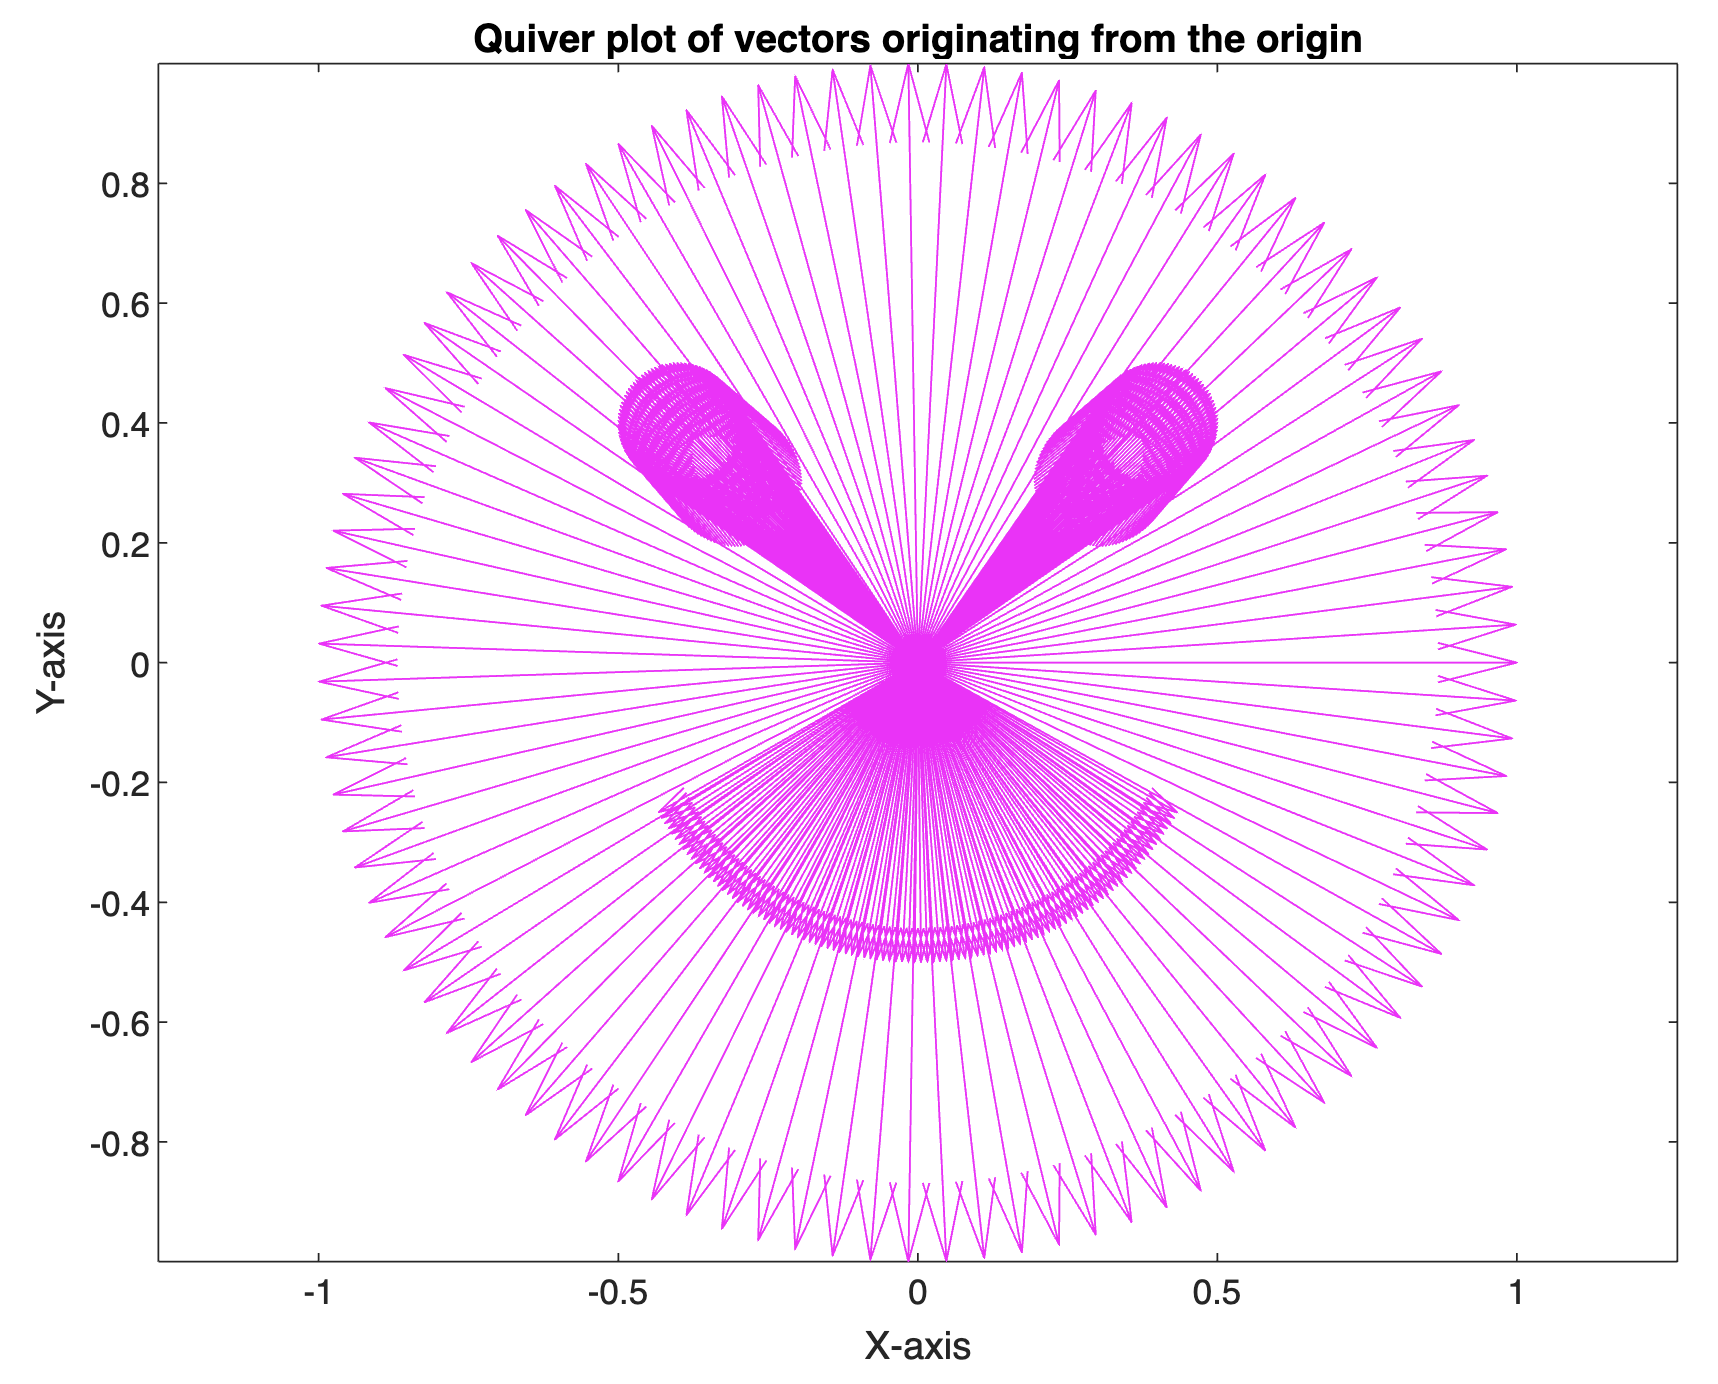
\includegraphics[width=0.5\textwidth]{smiley2.png}
        \end{center}

    \end{remark}


        Let's suppose that we had instead been given this plot of the smiley face to begin with:

        \begin{center}
            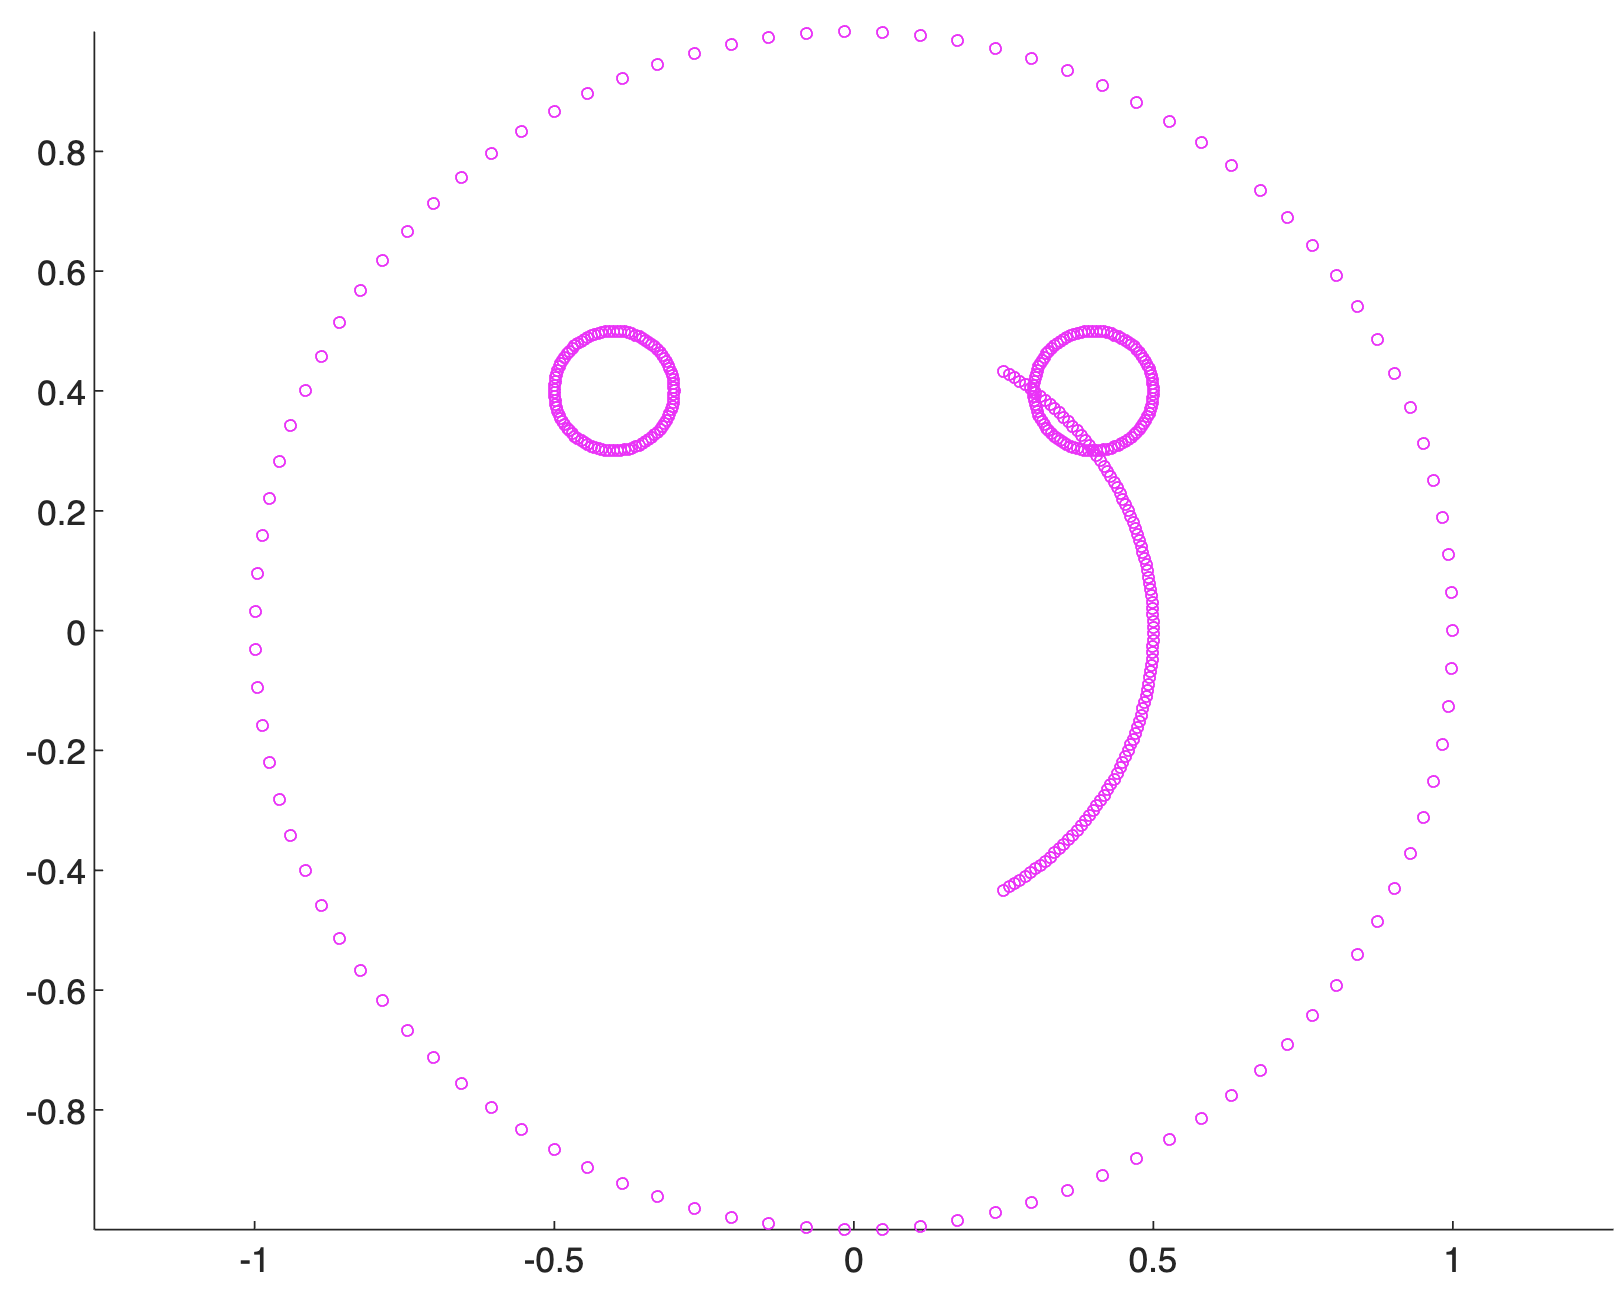
\includegraphics[width=0.5\textwidth]{smiley3.png}
        \end{center}

        We ca immediately see what's wrong with the picture, the smile part of the face has been rotated by 90 degrees. Our goal is to find a way to rotate the smile back, so that it makes the original image.

        We'll start with figuring out how to rotate a single vector, because what you can do to one, you can do to all of them.

    \begin{example}\name{Linear Combinations and Transformation}

        While we can use trigonometry to find an explicit function for rotatinge vectors, say by converting the cooridnates to angles and then further rotating to yeild new coordinates under the desired rotation, we can take a much simpler approach using the key tools of linear algebra, linear combinations.

        We already know that we can reprsent vectors as linear combinations of basis vectors (or more generally of spanning vectors). The typical starting point for any transformation (such as rotations) is to consider the standard basis vectors. For our purposes of planar images, we'll work with $\vec{i} = \begin{bmatrix} 1 \\ 0 \end{bmatrix}$ and $\vec{j} = \begin{bmatrix} 0 \\ 1 \end{bmatrix}$.

        To rotate $\vec{i}$ by some angle $\theta$, its new coordinates depend on the sine and cosine of $\theta$, so if for now we consider our rotation function $r$ to be a rotation by $\theta$, then we can write $r(\vec{i}) = \begin{bmatrix} \cos\theta \\ \sin\theta \end{bmatrix}$.

        Since $\vec{j}$ starts at $\begin{bmatrix} 0 \\ 1 \end{bmatrix}$, we rotate the triangle from its usual orientation to instead start along the $y$-axis. Since the legs of both triangles have the same lengths, we can still use $\sin(\theta)$ and $\cos(\theta)$ to determine the lengths of the new triangle, however we re-interpret their meaning with respect to their position in space. With this new triangle, the horizontal component length is found by $\sin(\theta)$, but since it moves backwards we need to use $-\sin(\theta)$. The vertical component is now found by $\cos(\theta)$, and is still positive. Thus, $r(\vec{j}) = \begin{bmatrix} -\sin\theta \\ \cos\theta \end{bmatrix}$.

        The rotations of these vectors are shown in the figure below:


        \begin{center}
        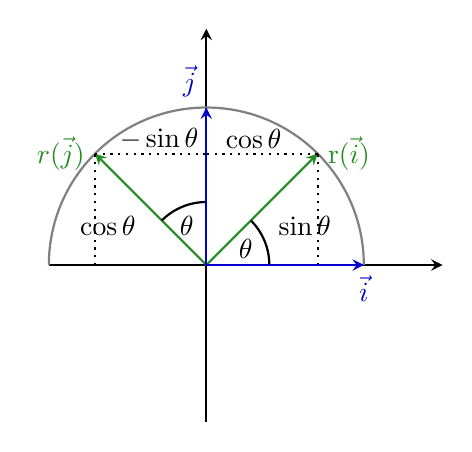
\begin{tikzpicture}

            % Define colors
            \definecolor{greenvec}{RGB}{34,139,34}
            \definecolor{bluevec}{RGB}{0,0,205}
            
            % Draw axes
            \draw[->, thick] (-2,0) -- (3,0); %node[right] {$\hat{e}_x$};
            \draw[->, thick] (0,-2) -- (0,3); %node[above] {$\hat{e}_y$};
            
            % Draw circle (semi-circle)
            \draw[gray, thick] (2,0) arc[start angle=0,end angle=180,radius=2];
            
            % Draw rotated vectors e_x' and e_y'
            \draw[->, thick, greenvec] (0,0) -- ({2*cos(45)},{2*sin(45)}) node[right] {r($\vec{i})$};
            \draw[->, thick, greenvec] (0,0) -- ({-2*sin(45)},{2*cos(45)}) node[left] {$r(\vec{j})$};
            
            % Dotted lines for projections
            \draw[dotted, thick] ({2*cos(45)},0) -- ({2*cos(45)},{2*sin(45)});
            \draw[dotted, thick] ({-2*sin(45)},0) -- ({-2*sin(45)},{2*cos(45)});
            \draw[dotted, thick] ({2*cos(45)},{2*sin(45)}) -- (0,{2*sin(45)});
            \draw[dotted, thick] ({-2*sin(45)},{2*cos(45)}) -- (0,{2*cos(45)});
            
            % Label angles and sin/cos values
            \draw (0.5,0.2) node {$\theta$};
            \draw (.6,1.6) node {$\cos\theta$};
            \draw (1.25,0.5) node {$\sin\theta$};
            \draw (-.6,1.6) node {$-\sin\theta$};
            \draw (-1.25,.5) node {$\cos\theta$};
            \draw (-.25,.5) node {$\theta$};
            
            % Angle arc
            \draw[thick] (0.8,0) arc[start angle=0, end angle=45, radius=0.8];
            \draw[thick] (0,.8) arc[start angle=90, end angle=135, radius=0.8];
            
            % Original basis vectors
            \draw[->, thick, bluevec] (0,0) -- (2,0) node[below] {$\vec{i}$};
            \draw[->, thick, bluevec] (0,0) -- (0,2) node[above left] {$\vec{j}$};
            
            \end{tikzpicture}
        \end{center}

        We could move from here and get more complicated, breaking down each possible vector into sines and cosines and re-interpreting the fundamental right-triangle trigonometry, OR we can make use of linear combinations to do the hard work for us.

        As it turns out, if our original vector $\vec{v}=a\vec{i}+b\vec{j}$, then we can find the rotation of $\vec{v}$ by first rotating $\vec{i}$ and $\vec{j}$, and then using the same scalars $a$ and $b$ to construct the rotated vector $r(\vec{v}) = a \cdot r(\vec{i}) + b \cdot r(\vec{j})$.

        Try it out on a few vectors using the following GeoGebra applet:

        First enter where you want the new basis vectors to go after rotation. For $90^\circ$ rotation, $r(\vec{i})$ should be $\begin{bmatrix} 0 \\ 1 \end{bmatrix}$ and $r(\vec{j})$ should be $\begin{bmatrix} -1 \\ 0 \end{bmatrix}$.

        Then, check the "Track Vector Transformation" box and move the vector $\vec{v}$ to a location of our choosing. Hitting the "Apply Linear Transformation" button will rotate the vector by $90^\circ$, and will display the resulting linear combination of the rotated basis vectors.

        \begin{center}
            \geogebra{wypahbvn}{809}{445}
        \end{center}

        Use the applet to find the rotations of the following vectors:

        \begin{enumerate}

            \item $\vec{v}=\begin{bmatrix} 1 \\ 1 \end{bmatrix}$ rotated by $60^\circ$ is (rounded to two decimal places) $\begin{bmatrix} \answer{-.37} \\ \answer{1.37} \end{bmatrix}$.
            
            \item $\vec{v}=\begin{bmatrix} 2 \\ 3 \end{bmatrix}$ rotated by $45^\circ$ is (rounded to two decimal places) $\begin{bmatrix} \answer{-.71} \\ \answer{3.54} \end{bmatrix}$.
            
            \item $\vec{v}=\begin{bmatrix} -1 \\ -2 \end{bmatrix}$ rotated by $30^\circ$ is (rounded to two decimal places) $\begin{bmatrix} \answer{.13} \\ \answer{-2.23} \end{bmatrix}$.
        \end{enumerate}

    \end{example}

    \begin{example}\name{Checking our Work}

        Let's verify that this works for a rotation that we know from the unit circle. If we start at an angle of $\theta = 45^\circ$, the associated vector is 
        
        $$\vec{v}=\begin{bmatrix} \frac{\sqrt{2}}{2} \\ \frac{\sqrt{2}}{2} \end{bmatrix}.$$

        If we rotate by $90^\circ$, we arrive at an angle of $135^\circ$, and the associated vector is 

        $$r(\vec{v}) = \begin{bmatrix} -\frac{\sqrt{2}}{2} \\ \frac{\sqrt{2}}{2} \end{bmatrix}.$$

        If our rotation function $r$ is correct, then we start at $\vec{v}$ so $a=\sqrt{2}/2$ and $b=\sqrt{2}/2$. Then we have for $90^\circ$ rotation, $r(\vec{i})=\begin{bmatrix} 0 \\ 1 \end{bmatrix}$ and $r(\vec{j})=\begin{bmatrix} -1 \\ 0 \end{bmatrix}$, so 

        $$r(\vec{v}) = \frac{\sqrt{2}}{2} \begin{bmatrix} 0 \\ 1 \end{bmatrix} + \frac{\sqrt{2}}{2} \begin{bmatrix} -1 \\ 0 \end{bmatrix} = \begin{bmatrix} -\frac{\sqrt{2}}{2} \\ \frac{\sqrt{2}}{2} \end{bmatrix}.$$

        Double check that this matches the rotation seen in the GeoGebra applet.

    \end{example}

    \begin{remark}

        This process of rotation gives us the foundation for building an entire collection of transformations on vectors (and one of the most important interpretations of matrices): The Linear Transformation.

        Our process of rotating vectors was:

        \begin{enumerate}

            \item Rotate the standard basis vectors.
        
            \item Write the original vector as a linear combination of the standard basis vectors.
            
            \item Use the same scalars to construct the new vector as a linear combination of the rotated basis vectors.
            
        \end{enumerate}

        As it turns out, this process defines a whole class of transformations, where we don't just rotate vectors, but can also stretch, shrink, reflect, shear, and more generally apply any kind of transformation we want, as long as we build it from basis vectors.

        \begin{definition}\name{Linear transformation}
            A vector function $T:\R^n\to \R^m$ is called a \textbf{linear
              transformation}%
            \index{linear transformation!on $\R^n$}, or simply \textbf{linear}, if it
            satisfies the following two conditions:
            \begin{enumerate}
            \item $T$ preserves addition, i.e., for all\/
              $\vect{v},\vect{w}\in\R^n$, we have
              $T(\vect{v}+\vect{w}) = T(\vect{v}) + T(\vect{w})$;
            \item $T$ preserves scalar multiplication, i.e, for all\/
              $\vect{v}\in\R^n$ and scalars $k$, we have
              $T(k\vect{v}) = kT(\vect{v})$.
            \end{enumerate}

            Said differently, linear transformations are built from linear combinations of basis vectors.
          \end{definition}

        More importantly, this also gives us a key operation for matrices: matrix-vector multiplication. 

        If we interpret the columns of a matrix $A$ as the transformations of the standard basis vectors, then the product $A\vec{v}$ of $A$ with any vector $\vec{v}$ is the transformed vector of $\vec{v}$. From this, we define matrix-vector multiplcation in the following way:

        \begin{definition}\name{Matrix-Vector Multiplication}
            Let $A$ be an $m\times n$ matrix and $\vec{v}$ be a vector in $\R^n$. The product $A\vec{v}$ is the vector in $\R^m$ obtained from the following operations:
            
            \begin{enumerate}

                \item Form $n$ vectors in $\R^m$ from the columns of $A$, denoted $A\vec{e}_1, A\vec{e}_2, \ldots, A\vec{e}_n$. These are the transformed standard basis vectors of $\R^n$, $\vec{e}_1, \vec{e}_2, \ldots, \vec{e}_n$.
                
                \item Form $n$ scalars $v_1, v_2, \ldots, v_n$ from the entries of $\vec{v}$.
                
                \item Build $A\vec{v}$ as the linear combination of the transformed standard basis vectors:
                
                $$A\vec{v} = v_1A\vec{e}_1 + v_2A\vec{e}_2 + \cdots + v_nA\vec{e}_n.$$

            \end{enumerate}
        \end{definition}

        Unlike scalar multiplication, matrix-vector multiplication requires that the column dimension of the matrix matches the vector dimension, and guarantees that the resulting vector's dimension matches the row dimension of the matrix. This means that matrix-vector multiplication won't always be possible for any pair of matrices and vectors.

        \begin{example}

            Verify that the rotations calculated from the GeoGebra applet are the same as the matrix-vector multiplication of the rotation matrix $R$ with the vectors $\vec{v}$.

            Since the rotation matrix $R$ has columns taken from the rotation function, we can write $R=\left[r(\vec{e}_1), r(\vec{e}_2)\right]=\begin{bmatrix} \cos\theta & -\sin\theta \\ \sin\theta & \cos\theta \end{bmatrix}$.

            Let's first do a quick check with MATLAB, which already has a built-in matrix-vector multiplication using the $\texttt{A*v}$ command. We'll use the rotation matrix $R$ for a $60^\circ$ rotation, and the vector $\vec{v}=\begin{bmatrix} 1 \\ 1 \end{bmatrix}$ from the previous example. 

            Running the code

            \begin{verbatim}
                theta=60;
                R = [cosd(60) -sind(60); sind(60) cosd(60)];
                v = [1; 1];
                R*v
            \end{verbatim}

            yeilds $\begin{bmatrix} -.37 \\ 1.37 \end{bmatrix}$, which matches the rotation calculated from the GeoGebra applet.

            In the following, write out the rotation matrix $R$, the transformed basis vectors $R\vec{e}_1$ and $R\vec{e}_2$, and the scalars in the linear combination that verify the earlier calculations.

            \begin{enumerate}

                \item For a $45^\circ$ rotation, the rotation matrix $R$ is $\begin{bmatrix} \cos 45 & -\sin 45 \\ \sin 45 & \cos 45 \end{bmatrix} = \begin{bmatrix} \frac{\sqrt{2}}{2} & -\frac{\sqrt{2}}{2} \\ \frac{\sqrt{2}}{2} & \frac{\sqrt{2}}{2} \end{bmatrix}$.
                
                The matrix-vector product $A\vec{v}$, where $\vec{v}=\begin{bmatrix} 2 \\ 3 \end{bmatrix}$, is (use 2 decimal places) $A\vec{v}=\answer{2}\begin{bmatrix} \answer{.71} \\ \answer{.71} \end{bmatrix} + \answer{3}\begin{bmatrix} \answer{-.71} \\ \answer{.71} \end{bmatrix} = \begin{bmatrix} -.71 \\ 3.54 \end{bmatrix}$, just as we calculated earlier.

                \item For a $30^\circ$ rotation, the rotation matrix $R$ is $\begin{bmatrix} \cos 30 & -\sin 30 \\ \sin 30 & \cos 30 \end{bmatrix} = \begin{bmatrix} \frac{\sqrt{3}}{2} & -\frac{1}{2} \\ \frac{1}{2} & \frac{\sqrt{3}}{2} \end{bmatrix}$.
                
                The matrix-vector product $A\vec{v}$, where $\vec{v}=\begin{bmatrix} -1 \\ -2 \end{bmatrix}$, is (use 2 decimal places) $A\vec{v}=\answer{-1}\begin{bmatrix} \answer{.87} \\ \answer{.5} \end{bmatrix} + \answer{-2}\begin{bmatrix} \answer{-.5} \\ \answer{.87} \end{bmatrix} = \begin{bmatrix} .13 \\ -2.23 \end{bmatrix}$, just as we calculated earlier.
            \end{enumerate}

            \begin{hint}
            
                If you want to try out basic rotations from both definitions in a MATLAB file, find the $\texttt{mod\_2\_matrix\_trans.mlx}$ live script in the course files.

            \end{hint}

        \end{example}

    \end{remark}

    \begin{example}\name{Rotating the Smile}

        After all of this work, we can finally return to the original problem of rotating the smiley face back to its original orientation.

        All of the smile vectors are $2$-dimensional, so we just need to use a $2\times 2$ rotation matrix to rotate them back. The rotation matrix for a $-90$ degree rotation is $R=\begin{bmatrix} 0 & -1 \\ 1 & 0 \end{bmatrix}$.

        Try it for yourself in the $\texttt{mod\_2\_matrix\_trans.mlx}$ live script. The code is as follows:
        \begin{enumerate}

            \item Load the smiley face with the rotated smile and view the matrices $\texttt{face\_points}$ and $\texttt{smile\_points}$. (Remember that a matrix is an array of vectors, which is how we interpret both of these matrices).
            \begin{verbatim}
                load +linalg/separate_face_points.mat
                face_points
                smile_points
            \end{verbatim}

            \item Re-write each vector (row) $\vec{v}$ in $\texttt{smile\_points}$ as the rotated vector $R*\vec{v}$, where $R$ is the rotation matrix for a $-90$ degree rotation.
            
            \begin{verbatim}

                theta=-90
                R=[cosd(theta), -sind(theta);
                    sind(theta), cosd(theta)]
                for i=1:length(smile_points)
                    %NOTE: You need to transpose the vector in smile_points 
                    %so that the dimensions match, R is 2x2 and v is 1x2, 
                    %so we want v' the 2x1 transpose
                    smile_points(i,:)=R*smile_points(i,:)';
                end

            \end{verbatim}

            \item Check that the rotation worked!
            
            \begin{verbatim}
                linalg.plot_img_points(smile_points)
                hold on
                linalg.plot_img_points(face_points)
                hold off
            \end{verbatim}

        \end{enumerate}

        The resulting plot should show the smiley face with the smile back in its original orientation.

    \end{example}

\end{exploration}

\begin{exploration}\name{Other Useful Transformation Matrices}

    While rotations are common, and actually quite important, there are plenty of other useful transformations that are usefl to know. These also give great opportunities to practice writing linear transformations as matrix-vector products!

    You'll go over these in more detail during the discussion activity, but here is an overview of some of the more common transformations.

    \begin{example}\name{Common Transformations}

        We'll now examine other commonly-used linear transformations that have nice properties. These transfromations are useful in computer graphics, physics, and other fields. 

        All of these transformations have $3$-dimensional analogues, but we'll start with the $2$-dimensional versions.

        Remember that the most important information for a linear transformation is how it transforms the standard basis vectors.

        \begin{enumerate}

            \item {\bf Reflection:} Let $T:\R^2\to\R^2$ be a reflection about the $y$-axis. Find the
            matrix%
            \index{matrix!of a reflection}%
            \index{reflection!matrix of}%
            \index{linear transformation!reflection} $A$ corresponding to this
            linear transformation, and a formula for $T$.
          
          \begin{solution}
            The before-and-after picture for a reflection about the $y$-axis
            looks like this:
            \begin{center}
              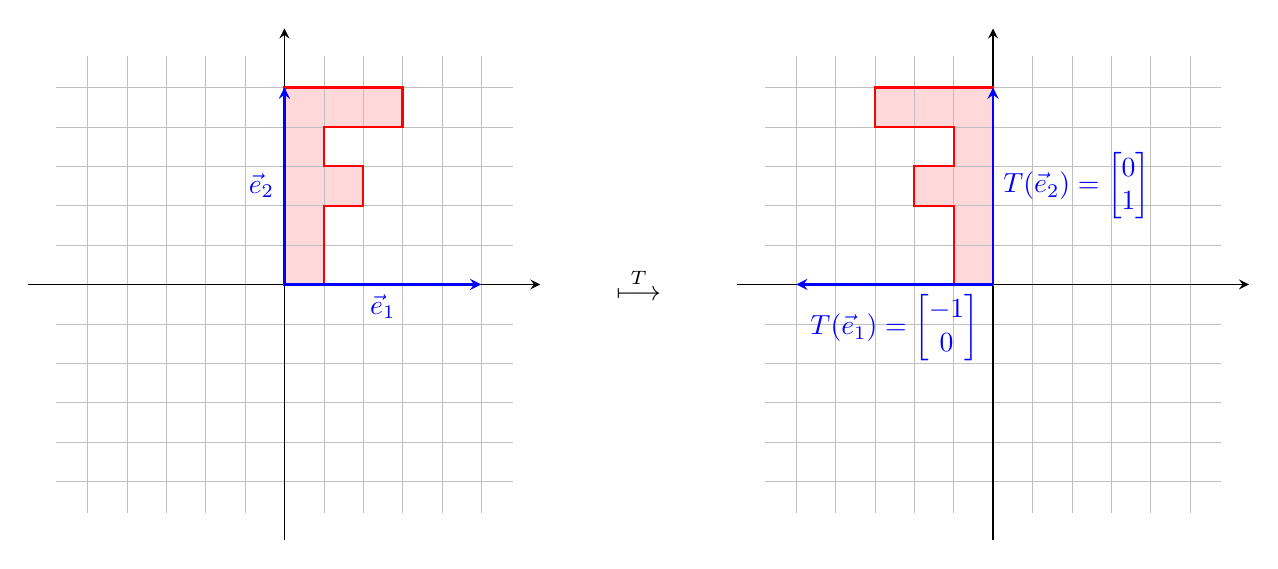
\begin{tikzpicture}
                \begin{scope}[scale=0.5]
                  \draw[red,thick,fill=red!15]
                  (0,0) -- (0,5) -- (3,5) -- (3,4) -- (1,4) --
                  (1,3) -- (2,3) -- (2,2) -- (1,2) -- (1,0) -- cycle;
                  \draw[step=1cm, gray!50, very thin] (-5.8,-5.8) grid (5.8,5.8);
                  \draw[semithick,->] (-6.5,0) -- (6.5,0);
                  \draw[semithick,->] (0,-6.5) -- (0,6.5);
                  \draw[red,thick]
                  (0,0) -- (0,5) -- (3,5) -- (3,4) -- (1,4) --
                  (1,3) -- (2,3) -- (2,2) -- (1,2) -- (1,0) -- cycle;
                  \draw[blue,thick,->] (0,0) -- node[below] {$\vect{e}_1$} (5,0);
                  \draw[blue,thick,->] (0,0) -- node[left] {$\vect{e}_2$} (0,5);
                \end{scope}
                \begin{scope}[xshift=4.5cm]
                  \path (0,0) node {$\stackrel{T}{\longmapsto}$};
                \end{scope}
                \begin{scope}[xshift=9cm,scale=0.5]
                  \draw[red,thick,fill=red!15,xscale=-1]
                  (0,0) -- (0,5) -- (3,5) -- (3,4) -- (1,4) --
                  (1,3) -- (2,3) -- (2,2) -- (1,2) -- (1,0) -- cycle;
                  \draw[step=1cm, gray!50, very thin] (-5.8,-5.8) grid (5.8,5.8);
                  \draw[semithick,->] (-6.5,0) -- (6.5,0);
                  \draw[semithick,->] (0,-6.5) -- (0,6.5);
                  \draw[red,thick,xscale=-1]
                  (0,0) -- (0,5) -- (3,5) -- (3,4) -- (1,4) --
                  (1,3) -- (2,3) -- (2,2) -- (1,2) -- (1,0) -- cycle;
                  \draw[blue,thick,->,xscale=-1] (0,0) -- node[below]
                  {$T(\vect{e}_1) = \begin{bmatrix}-1\\0\end{bmatrix}$}
                  (5,0);
  \draw[blue,thick,->,xscale=-1] (0,0) --
                  node[right] {$T(\vect{e}_2) = \begin{bmatrix}0\\1\end{bmatrix}$}
                  (0,5);
                \end{scope}
              \end{tikzpicture}
            \end{center}
            We see that
            \begin{equation*}
              T(\vect{e}_1) = -\vect{e}_1 = \begin{bmatrix}-1\\0\end{bmatrix}
              \quad\mbox{and}\quad
              T(\vect{e}_2) = \vect{e}_2 = \begin{bmatrix}0\\1\end{bmatrix}.
            \end{equation*}
            Therefore, the matrix of $T$ is
            \begin{equation*}
              A = \begin{bmatrix}
                -1 & 0 \\
                0  & 1 \\
              \end{bmatrix}.
            \end{equation*}
          \end{solution}

          \item We describe the linear transformation that is given by each of the
            following matrices in terms of reflections, rotations, and scalings:
            \begin{enumerate}
                \item 
            \begin{equation*}
              \quad
              A = \begin{bmatrix}
                0 & 1 \\
                1 & 0 \\
              \end{bmatrix}
            \end{equation*}

            \begin{solution}
                To draw each before-and-after picture, we can start by drawing the
                images of the two standard basis vectors $\vec{e}_1$ and
                $\vec{e}_2$, which are the columns of the transformation matrix. We
                have also drawn the image of the letter ``F'', to better illustrate
                the effect of each transformation.
                \begin{center}
                  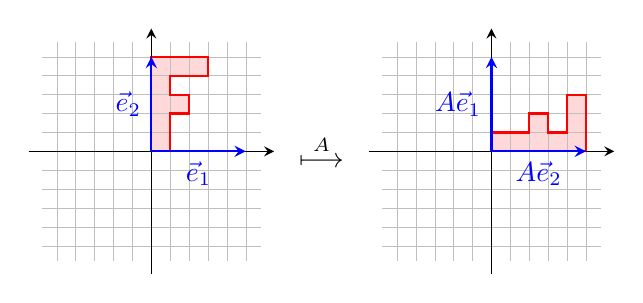
\begin{tikzpicture}[scale=0.96]
                    \begin{scope}

                      \begin{scope}[scale=0.25]
                        \draw[red,thick,fill=red!15]
                        (0,0) -- (0,5) -- (3,5) -- (3,4) -- (1,4) --
                        (1,3) -- (2,3) -- (2,2) -- (1,2) -- (1,0) -- cycle;
                        \draw[step=1cm, gray!50, very thin] (-5.8,-5.8) grid (5.8,5.8);
                        \draw[red,thick]
                        (0,0) -- (0,5) -- (3,5) -- (3,4) -- (1,4) --
                        (1,3) -- (2,3) -- (2,2) -- (1,2) -- (1,0) -- cycle;
                        \draw[semithick,->] (-6.5,0) -- (6.5,0);
                        \draw[semithick,->] (0,-6.5) -- (0,6.5);
                        \draw[blue,thick,->] (0,0) -- node[below] {$\vec{e}_1$} (5,0);
                        \draw[blue,thick,->] (0,0) -- node[left] {$\vec{e}_2$} (0,5);
                      \end{scope}
                      \begin{scope}[xshift=2.25cm]
                        \path (0,0) node {$\stackrel{A}{\longmapsto}$};
                      \end{scope}
                      \begin{scope}[xshift=4.5cm,scale=0.25]
                        \draw[red,thick,fill=red!15,cm={0,1,1,0,(0,0)}]
                        (0,0) -- (0,5) -- (3,5) -- (3,4) -- (1,4) --
                        (1,3) -- (2,3) -- (2,2) -- (1,2) -- (1,0) -- cycle;
                        \draw[step=1cm, gray!50, very thin] (-5.8,-5.8) grid (5.8,5.8);
                        \draw[red,thick,cm={0,1,1,0,(0,0)}]
                        (0,0) -- (0,5) -- (3,5) -- (3,4) -- (1,4) --
                        (1,3) -- (2,3) -- (2,2) -- (1,2) -- (1,0) -- cycle;
                        \draw[semithick,->] (-6.5,0) -- (6.5,0);
                        \draw[semithick,->] (0,-6.5) -- (0,6.5);
                        \draw[blue,thick,->,cm={0,1,1,0,(0,0)}] (0,0) --
                        node[left] {$A\vec{e}_1$} (5,0);
                        \draw[blue,thick,->,cm={0,1,1,0,(0,0)}] (0,0) --
                        node[below] {$A\vec{e}_2$} (0,5);
                      \end{scope}
                    \end{scope}
                \end{tikzpicture}
                \end{center}

                The transformation $A$ is a reflection%
                \index{matrix!of a reflection}%
                \index{reflection!matrix of}%
                \index{linear transformation!reflection} about the line $x=y$. 

                You might also describe the effect as swapping the positions of the standard basis vectors. This kind of transformation will be important in the next chapter. 
            \end{solution}

        \item 
            \begin{equation*}
              \quad
              B = \begin{bmatrix}
                2 & 0 \\
                0 & 2 \\
              \end{bmatrix},\quad
            \end{equation*}

            \begin{solution}
                \begin{center}
                    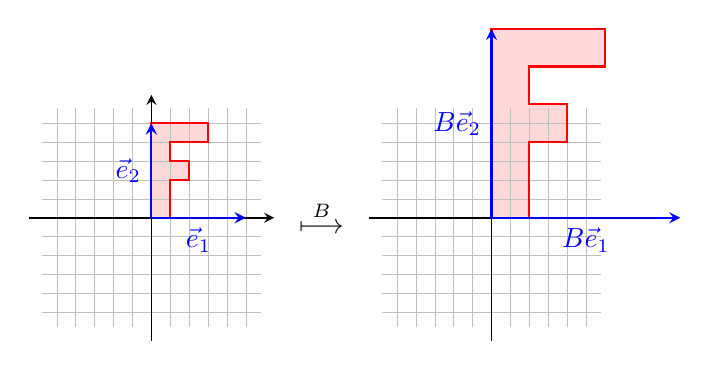
\begin{tikzpicture}[scale=0.96]
                    \begin{scope}[xshift=9cm]
                      \begin{scope}[scale=0.25]
                        \draw[red,thick,fill=red!15]
                        (0,0) -- (0,5) -- (3,5) -- (3,4) -- (1,4) --
                        (1,3) -- (2,3) -- (2,2) -- (1,2) -- (1,0) -- cycle;
                        \draw[step=1cm, gray!50, very thin] (-5.8,-5.8) grid (5.8,5.8);
                        \draw[red,thick]
                        (0,0) -- (0,5) -- (3,5) -- (3,4) -- (1,4) --
                        (1,3) -- (2,3) -- (2,2) -- (1,2) -- (1,0) -- cycle;
                        \draw[semithick,->] (-6.5,0) -- (6.5,0);
                        \draw[semithick,->] (0,-6.5) -- (0,6.5);
                        \draw[blue,thick,->] (0,0) -- node[below] {$\vec{e}_1$} (5,0);
                        \draw[blue,thick,->] (0,0) -- node[left] {$\vec{e}_2$} (0,5);
                      \end{scope}
                      \begin{scope}[xshift=2.25cm]
                        \path (0,0) node {$\stackrel{B}{\longmapsto}$};
                      \end{scope}
                      \begin{scope}[xshift=4.5cm,scale=0.25]
                        \draw[red,thick,fill=red!15,cm={2,0,0,2,(0,0)}]
                        (0,0) -- (0,5) -- (3,5) -- (3,4) -- (1,4) --
                        (1,3) -- (2,3) -- (2,2) -- (1,2) -- (1,0) -- cycle;
                        \draw[step=1cm, gray!50, very thin] (-5.8,-5.8) grid (5.8,5.8);
                        \draw[red,thick,cm={2,0,0,2,(0,0)}]
                        (0,0) -- (0,5) -- (3,5) -- (3,4) -- (1,4) --
                        (1,3) -- (2,3) -- (2,2) -- (1,2) -- (1,0) -- cycle;
                        \draw[semithick] (-6.5,0) -- (6.5,0);
                        \draw[semithick] (0,-6.5) -- (0,6.5);
                        \draw[blue,thick,->,cm={2,0,0,2,(0,0)}] (0,0) --
                        node[below] {$B\vec{e}_1$} (5,0);
                        \draw[blue,thick,->,cm={2,0,0,2,(0,0)}] (0,0) --
                        node[left] {$B\vec{e}_2$} (0,5);
                      \end{scope}
                    \end{scope}
                    \end{tikzpicture}
                \end{center}

                The
                transformation $B$ is a scaling%
                \index{matrix!of a scaling}%
                \index{scaling!matrix of}%
                \index{linear transformation!scaling} by a factor of $2$. 
    
            \end{solution}

        \item 
        \begin{equation*}
            C = \begin{bmatrix}
              \frac{1}{2} & 0 \\
              0 & 2 \\
            \end{bmatrix}
        \end{equation*}

            \begin{solution}
                \begin{center}
                    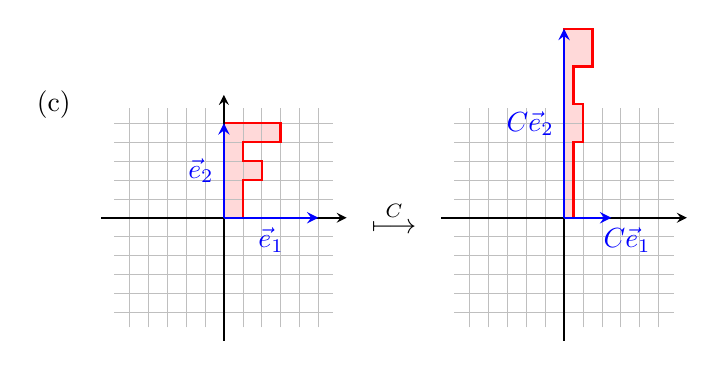
\begin{tikzpicture}[scale=0.96]
                    \begin{scope}[yshift=-3.75cm]
                      \path (-2.25,1.5) node {(c)};
                      \begin{scope}[scale=0.25]
                        \draw[red,thick,fill=red!15]
                        (0,0) -- (0,5) -- (3,5) -- (3,4) -- (1,4) --
                        (1,3) -- (2,3) -- (2,2) -- (1,2) -- (1,0) -- cycle;
                        \draw[step=1cm, gray!50, very thin] (-5.8,-5.8) grid (5.8,5.8);
                        \draw[red,thick]
                        (0,0) -- (0,5) -- (3,5) -- (3,4) -- (1,4) --
                        (1,3) -- (2,3) -- (2,2) -- (1,2) -- (1,0) -- cycle;
                        \draw[semithick,->] (-6.5,0) -- (6.5,0);
                        \draw[semithick,->] (0,-6.5) -- (0,6.5);
                        \draw[blue,thick,->] (0,0) -- node[below] {$\vec{e}_1$} (5,0);
                        \draw[blue,thick,->] (0,0) -- node[left] {$\vec{e}_2$} (0,5);
                      \end{scope}
                      \begin{scope}[xshift=2.25cm]
                        \path (0,0) node {$\stackrel{C}{\longmapsto}$};
                      \end{scope}
                      \begin{scope}[xshift=4.5cm,scale=0.25]
                        \draw[red,thick,fill=red!15,cm={0.5,0,0,2,(0,0)}]
                        (0,0) -- (0,5) -- (3,5) -- (3,4) -- (1,4) --
                        (1,3) -- (2,3) -- (2,2) -- (1,2) -- (1,0) -- cycle;
                        \draw[step=1cm, gray!50, very thin] (-5.8,-5.8) grid (5.8,5.8);
                        \draw[red,thick,cm={0.5,0,0,2,(0,0)}]
                        (0,0) -- (0,5) -- (3,5) -- (3,4) -- (1,4) --
                        (1,3) -- (2,3) -- (2,2) -- (1,2) -- (1,0) -- cycle;
                        \draw[semithick,->] (-6.5,0) -- (6.5,0);
                        \draw[semithick] (0,-6.5) -- (0,6.5);
                        \draw[blue,thick,->,cm={0.5,0,0,2,(0,0)}] (0,0) --
                        node[below,xshift=0.5cm] {$C\vec{e}_1$} (5,0);
                        \draw[blue,thick,->,cm={0.5,0,0,2,(0,0)}] (0,0) --
                        node[left] {$C\vec{e}_2$} (0,5);
                      \end{scope}
                    \end{scope}
                    \end{tikzpicture}
                \end{center}

                The
                transformation $C$ is also a scaling, but by a different factor in
                the $x$- and $y$-directions. It scales the $x$-direction by a factor
                of $\frac{1}{2}$ (or equivalently, shrinks it by a factor of $2$),
                and scales the $y$-direction by a factor of $2$. 

            \end{solution}

            \item 
        \begin{equation*}
              D = \begin{bmatrix}
                1 & 1 \\
                0 & 1 \\
              \end{bmatrix}.
            \end{equation*}
          
        
        \begin{solution}
            \begin{center}
                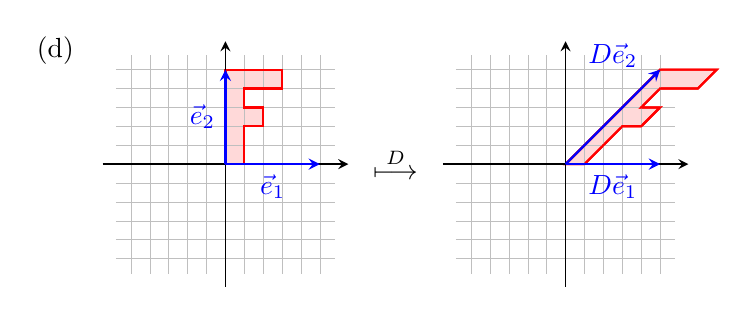
\begin{tikzpicture}[scale=0.96]
                \begin{scope}[xshift=9cm,yshift=-3.75cm]
                  \path (-2.25,1.5) node {(d)};
                  \begin{scope}[scale=0.25]
                    \draw[red,thick,fill=red!15]
                    (0,0) -- (0,5) -- (3,5) -- (3,4) -- (1,4) --
                    (1,3) -- (2,3) -- (2,2) -- (1,2) -- (1,0) -- cycle;
                    \draw[step=1cm, gray!50, very thin] (-5.8,-5.8) grid (5.8,5.8);
                    \draw[red,thick]
                    (0,0) -- (0,5) -- (3,5) -- (3,4) -- (1,4) --
                    (1,3) -- (2,3) -- (2,2) -- (1,2) -- (1,0) -- cycle;
                    \draw[semithick,->] (-6.5,0) -- (6.5,0);
                    \draw[semithick,->] (0,-6.5) -- (0,6.5);
                    \draw[blue,thick,->] (0,0) -- node[below] {$\vec{e}_1$} (5,0);
                    \draw[blue,thick,->] (0,0) -- node[left] {$\vec{e}_2$} (0,5);
                  \end{scope}
                  \begin{scope}[xshift=2.25cm]
                    \path (0,0) node {$\stackrel{D}{\longmapsto}$};
                  \end{scope}
                  \begin{scope}[xshift=4.5cm,scale=0.25]
                    \draw[red,thick,fill=red!15,cm={1,0,1,1,(0,0)}]
                    (0,0) -- (0,5) -- (3,5) -- (3,4) -- (1,4) --
                    (1,3) -- (2,3) -- (2,2) -- (1,2) -- (1,0) -- cycle;
                    \draw[step=1cm, gray!50, very thin] (-5.8,-5.8) grid (5.8,5.8);
                    \draw[red,thick,cm={1,0,1,1,(0,0)}]
                    (0,0) -- (0,5) -- (3,5) -- (3,4) -- (1,4) --
                    (1,3) -- (2,3) -- (2,2) -- (1,2) -- (1,0) -- cycle;
                    \draw[semithick,->] (-6.5,0) -- (6.5,0);
                    \draw[semithick,->] (0,-6.5) -- (0,6.5);
                    \draw[blue,thick,->,cm={1,0,1,1,(0,0)}] (0,0) --
                    node[below] {$D\vec{e}_1$} (5,0);
                    \draw[blue,thick,->,cm={1,0,1,1,(0,0)}] (0,0) --
                    node[above,yshift=0.5cm] {$D\vec{e}_2$} (0,5);
                  \end{scope}
                \end{scope}
              \end{tikzpicture}
            \end{center}

            The transformation
            $D$ is called a \textbf{shearing}%
            \index{matrix!of a shearing}%
            \index{shearing!matrix of}%
            \index{linear transformation!shearing}. It keeps one line (the
            $x$-axis) fixed, while shifting all other points by varying
            distances along lines that are parallel to the $x$-axis.

          \end{solution}
        \end{enumerate}

        \item somthing 3D

        \end{enumerate}

    \end{example}

\end{exploration}

\begin{exploration}\name{Sequencing Transformations - Matrix Multiplication}

    We've now got a good handle on performing singular transformations of vectors using matrices. But what if we want to perform multiple transformations on a vector?

    Suppose we wanted to take our original smiley face, stretch it out in the vertical direction, rotate it $60^\circ$, and then reflect it about the $y$-axis. 

    We could do this in two ways:
    \begin{enumerate}

        \item Perform each transformation one at a time, and then apply the next transformation to the result.
        
        \item Determine the transformations of the standard basis vectors for the entire sequence, and use that single matrix to transform the original smiley face.

    \end{enumerate}

    Both of these procedures will get us the same final transformation, and using the first method to figure out the second method gives us another key operation: matrix-matrix multiplication (also just called matrix multiplication).

    Let's take each step in sequence, track the smiley face along the way, and use the steps together to make a final transformation. 

    \begin{example}

        Let's figure out how to do the first two operations in sequence, first a vertical stretch by a factor of $2$, and then a $60^\circ$ rotation.

        We know that a vertical stretch by a factor of $2$ is given by the matrix $S=\begin{bmatrix} 1 & 0 \\ 0 & 2 \end{bmatrix}$, and a $60^\circ$ rotation is given by the matrix $R=\begin{bmatrix} \cos 60 & -\sin 60 \\ \sin 60 & \cos 60 \end{bmatrix}$.

        Doing the two transformations in tandem means first applying the stretch, then applying the rotation \emph{on the stretched smiley face}.

        Let's first do each transformation in MATLAB, first the vertical stretch. For ease, we'll first load a separate file called $\texttt{face\_points.mat}$ that contains the smiley face points as a single matrix.

        \begin{verbatim}

            load +linalg/face_points.mat
        
            S = [1 0; 0 2];
            for i=1:length(face_points)
                face_points(i,:)=S*face_points(i,:)';
            end
            linalg.plot_img_points(face_points)

        \end{verbatim}

        That should yield a smiley face that is stretched vertically by a factor of $2$.

        \begin{center}
            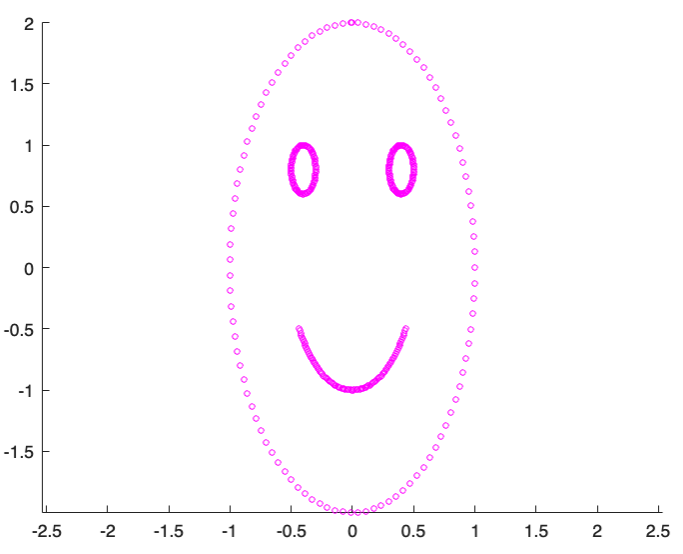
\includegraphics[width=0.75\textwidth]{face_stretch.png}
        \end{center}

        Next, if we just re-load $\texttt{face\_points}$ and run the same code (but for a rotation matrix), we won't keep the stretching. We would just get a $60^\circ$ rotation of the original smiley face like below.

        \begin{verbatim}

            R = [cosd(60) -sind(60); sind(60) cosd(60)];
            for i=1:length(face_points)
                face_points(i,:)=R*face_points(i,:)';
            end
            linalg.plot_img_points(face_points)
        \end{verbatim}

        \begin{center}
            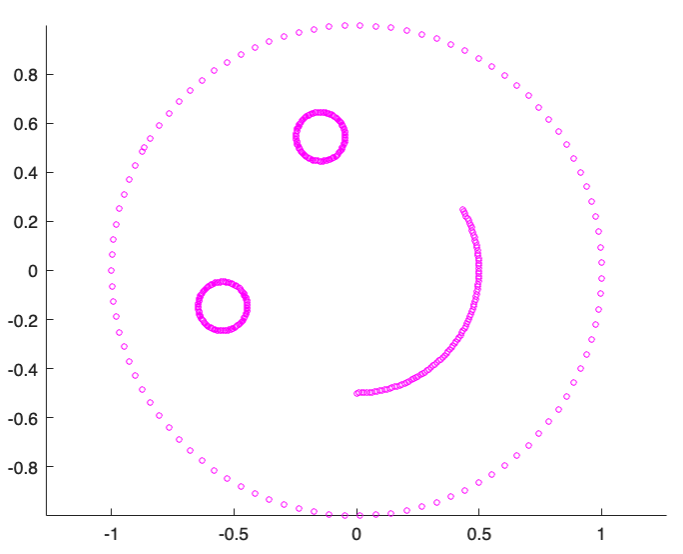
\includegraphics[width=.75\textwidth]{face_rotate.png}
        \end{center}

        Instead, we have to first apply the stretching, then keep the result and apply the rotation. 

        If we do one transformation and then the other right after, we could get the following: 

        \begin{verbatim}
                
                load +linalg/face_points.mat
    
                S = [1 0; 0 2];
                R = [cosd(60) -sind(60); sind(60) cosd(60)];
                for i=1:length(face_points)
                    face_points(i,:)=S*face_points(i,:)';
                end
                linalg.plot_img_points(face_points)

                for i=1:length(face_points)
                    face_points(i,:)=R*face_points(i,:)';
                end
                linalg.plot_img_points(face_points)
        \end{verbatim}

        Importantly, in between the for loops you see the intermediate stretching step. After the first loop, the vectors were all stretched, then they were further rotated in the second loop.

        This yeilds the following smiley faces:

        %do a side-by-side of the stretched and rotated smiley faces, within one single figure

        \begin{center}
            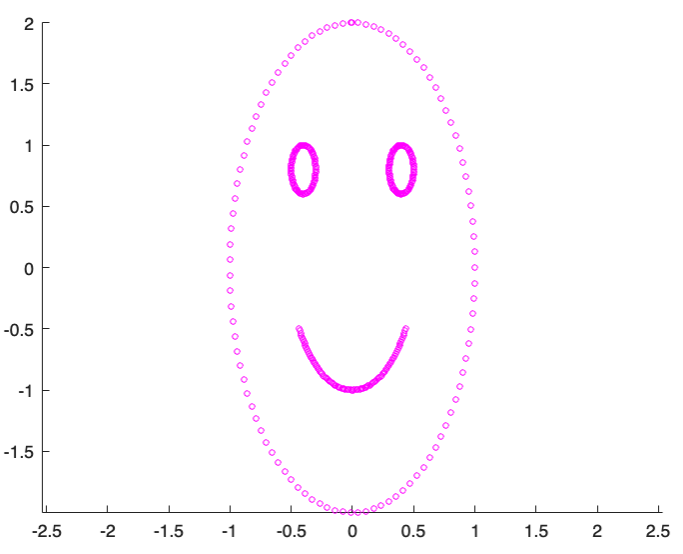
\includegraphics[width=.75\textwidth]{face_stretch.png}
        \end{center}

        \begin{center}
            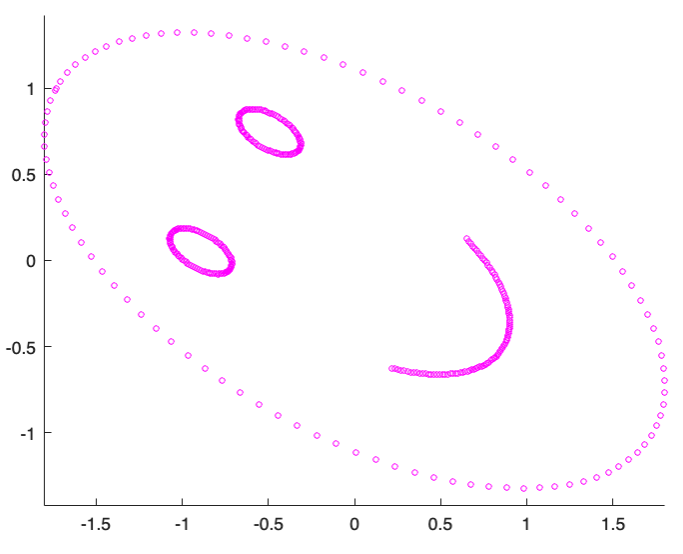
\includegraphics[width=.75\textwidth]{face_stretch_rotate.png}
        \end{center}

        The final smiley face is the result of the two transformations in sequence.

        \begin{remark}

        This is an example of what is called \emph{function composition}, where you chain multiple functions together in an input$\rightarrow$output$\rightarrow$input$\rightarrow$output sequence, progressively transforming the original inputs until you reach a final output.

        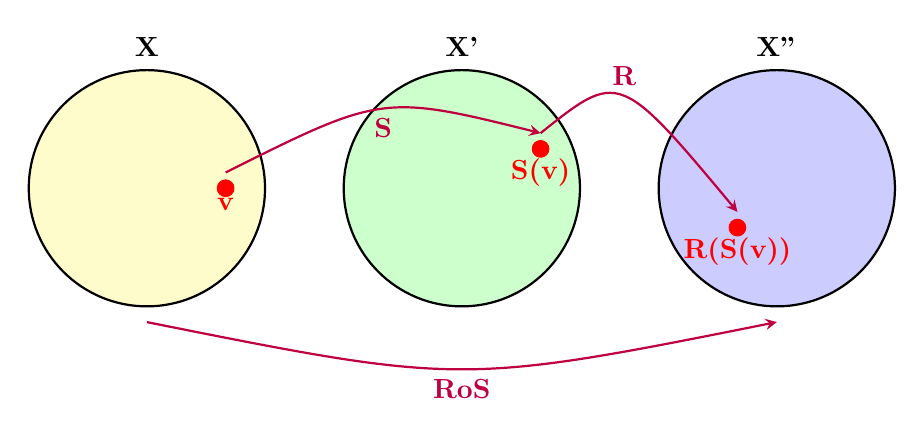
\begin{tikzpicture}

            % Draw sets A, B, C
            \draw[fill=yellow!20!white, draw=black, thick] (-4,0) ellipse (1.5cm);
            \draw[fill=green!20!white, draw=black, thick] (0,0) ellipse (1.5cm);
            \draw[fill=blue!20!white, draw=black, thick] (4,0) ellipse (1.5cm);
            
            % Labels for sets A, B, C
            \node at (-4,1.8) {\textbf{X}};
            \node at (0,1.8) {\textbf{X'}};
            \node at (4,1.8) {\textbf{X''}};
            
            % Elements inside sets
            \filldraw[red] (-3,0) circle (3pt) node[below] {\textbf{v}};
            \filldraw[red] (1,.5) circle (3pt) node[below] {\textbf{S(v)}};
            \filldraw[red] (3.5,-.5) circle (3pt) node[below] {\textbf{R(S(v))}};
            
            % Arrows for functions f, g, gof
            \draw[->, thick, purple] (-3,0.2) .. controls (-1,1.2) .. (1,.7) node[midway, below] {\textbf{S}};
            \draw[->, thick, purple] (1,.7) .. controls (2,1.5) .. (3.5,-.3) node[midway, above] {\textbf{R}};
            \draw[->, thick, purple] (-4,-1.7) .. controls (0,-2.5) .. (4,-1.7) node[midway, below] {\textbf{RoS}};
            
        \end{tikzpicture}

        In the above diagram, $X$ is the original data, $X'$ is the data after the stretching transformation, and $X''$ is the data after the rotation transformation. The arrows represent the transformations that progressively alter the data, and the final arrow represents the composition of the two transformations.

    \end{remark}

    Our goal is to find a systematic way of representing the composite transformation as a single matrix. From this example, let's track the transformations of the standard basis vectors.

    We start with the standard basis vectors $\vec{e}_1=\begin{bmatrix} 1 \\ 0 \end{bmatrix}$ and $\vec{e}_2=\begin{bmatrix} 0 \\ 1 \end{bmatrix}$, and apply the transformations in sequence.

    The stretching transformation matrix is $S=\begin{bmatrix} 1 & 0 \\ 0 & 2 \end{bmatrix}$, which tells us that the stretched basis vectors are $S\vec{e}_1=\begin{bmatrix}\answer{1} \\ 0 \end{bmatrix}$ and $S\vec{e}_2=\begin{bmatrix} 0 \\ \answer{2} \end{bmatrix}$.

    Whereas the rotation matrix $R=\begin{bmatrix} \cos 60 & -\sin 60 \\ \sin 60 & \cos 60 \end{bmatrix}$ would normally tell us where to map $\vec{e}_1$ and $\vec{e}_2$, to continue the tansformation we instead need to apply the matrix to $S\vec{e}_1$ and $S\vec{e}_2$.

    \begin{hint}\name{Notation}

        Don't let the notation fool you, $S\vec{e}_1$ and $S\vec{e}_2$ vectors, not matrices. Remember that multiplying a matrix by a vector gives you a transformed vector.

    \end{hint}

    \begin{question}

        What are the rotated vectors $RS\vec{e}_1$ and $RS\vec{e}_2$?

        \begin{solution}

            We have $S\vec{e}_1=\begin{bmatrix} 1 \\ 0 \end{bmatrix}$ and $S\vec{e}_2=\begin{bmatrix} 0 \\ 2 \end{bmatrix}$.

            Applying the rotation matrix $R$ to $S\vec{e}_1$ gives us $R(S\vec{e}_1)=\begin{bmatrix} \cos 60 & -\sin 60 \\ \sin 60 & \cos 60 \end{bmatrix}\begin{bmatrix} 1 \\ 0 \end{bmatrix}=\answer{1}\begin{bmatrix} \cos 60 \\ \sin 60 \end{bmatrix}+\answer{0}
            \begin{bmatrix} -\sin 60 \\ \cos 60 \end{bmatrix}=\begin{bmatrix} \cos 60 \\ \sin 60 \end{bmatrix}$.

            Applying the rotation matrix $R$ to $S\vec{e}_2$ gives us $R(S\vec{e}_2)=\begin{bmatrix} \cos 60 & -\sin 60 \\ \sin 60 & \cos 60 \end{bmatrix}\begin{bmatrix} 0 \\ 2 \end{bmatrix}=\answer{0}\begin{bmatrix} \cos 60 \\ \sin 60 \end{bmatrix}+\answer{2}
            \begin{bmatrix} -\sin 60 \\ \cos 60 \end{bmatrix}=\begin{bmatrix} -2\sin 60 \\ 2\cos 60 \end{bmatrix}$.

        \end{solution}

    \end{question}

    Putting this together, we see that the composite transformation matrix $RS$ is 
    
    $$RS=\begin{bmatrix} \cos 60 & -2\sin 60 \\ \sin 60 & 2\cos 60 \end{bmatrix}.$$

    Let's check that this matrix gives us the same result as the two transformations in sequence.

    Use the following MATLAB code to apply the composite transformation to the original smiley face.

    \begin{verbatim}

        load +linalg/face_points.mat

        RS = [cosd(60) -2*sind(60); sind(60) 2*cosd(60)];
        for i=1:length(face_points)
            face_points(i,:)=RS*face_points(i,:)';
        end
        linalg.plot_img_points(face_points)
    \end{verbatim}

    This yields the same smiley face as the two transformations in sequence!


    \end{example}

    \begin{remark}

        Note also that the notation we used to find the new basis vectors, $RS\vec{e}_1$ and $RS\vec{e}_2$ feels quite similar to notation used for scalar multiplication. For instance if $a=3$ and $b=4$ we would write $ab$ to mean $3\cdot 4$.

        This gives rise to the following definition of \emph{matrix multiplication}

        \begin{definition}

            Let $A$ be an $m\times n$ matrix and $B$ be an $n\times p$ matrix. The product $AB$ is an $m\times p$ matrix whose columns are given by 

            $$AB=\begin{bmatrix} A\vec{b}_1 & A\vec{b}_2 & \cdots & A\vec{b}_p \end{bmatrix}$$

            where $\vec{b}_1,\vec{b}_2,\ldots,\vec{b}_p$ are the columns of $B$.

        \end{definition}

        There is another, more standard definition of matrix multiplication that you'll often see in textbooks, which breaks down the operation for each entry rather than at each column. It's worth noting for efficiency, and that you'll see it in other contexts, however thinking about it as a column-wise operation is a good way to understand why matrix multiplication works the way it does.

        \begin{definition}\name{Entry-Wise Matrix Multiplication}

            Let $A$ be an $m\times n$ matrix and $B$ be an $n\times p$ matrix. The product $AB$ is an $m\times p$ matrix whose entries are given by 

            $$(AB)_{ij}=\sum_{k=1}^n A_{ik}B_{kj}.$$
        \end{definition}

    \end{remark}

    As usual, MATLAB has a built-in function for matrix multiplication, $\texttt{A*B}$, which will give you the same result as the column-wise definition of matrix multiplication. Let's check it on the previous example.

    \begin{example}

        Let's use MATLAB to check that the matrix $RS$ we found earlier is the same as the product of the matrices $R$ and $S$.

        \begin{verbatim}

            R = [cosd(60) -sind(60); sind(60) cosd(60)]
            S = [1 0; 0 2]
            RS = R*S
            RS
        \end{verbatim}

        This should yield the matrix $RS$ we found earlier, $\begin{bmatrix} \cos 60 & -2\sin 60 \\ \sin 60 & 2\cos 60 \end{bmatrix}$.
    \end{example}

    \begin{example}

        We're finally able to do all three of the transformations we initial set out to do: a vertical stretch by a factor of $2$, a $60^\circ$ rotation, and a reflection about the $y$-axis.

        Let's do it first in sequence, then as one transformation, and compare the results.

        \begin{enumerate}

            \item In Sequence: We already know the matrices for the stretch and rotation are $S=\begin{bmatrix} 1 & 0 \\ 0 & 2 \end{bmatrix}$ and $R=\begin{bmatrix} \cos 60 & -\sin 60 \\ \sin 60 & \cos 60 \end{bmatrix}$. The matrix for the reflection is $F=\begin{bmatrix} \answer{-1} & 0 \\ 0 & \answer{1} \end{bmatrix}$.
            
            Let's apply the transformations in sequence using MALTAB. 
            
            \begin{hint}\name{MATLAB}
            
            NOTE: The code will do it all in one for loop rather than three, but notice that each line within the for loop is applying each separate transformation to the smiley face points. 
            
            So first it will stretch the points, then the next line will rotate the already stretched points, then the next line will reflect the already stretched and rotated points.

            \end{hint}



            $\texttt{load +linalg/face\_points.mat}$

            $\texttt{S = [1 0; 0 2]}$

            $\texttt{R = [cosd(60) -sind(60); sind(60) cosd(60)]}$

            $\texttt{F = [-1 0; 0 1]}$

            $\texttt{for i=1:length(face\_points)}$

            $\texttt{    face\_points(i,:)=}\answer[format=string]{S}\texttt{*face\_points(i,:)';}$

            $\texttt{        face\_points(i,:)=}\answer[format=string]{R}\texttt{*face\_points(i,:)';}$

            $\texttt{        face\_points(i,:)=}\answer[format=string]{F}\texttt{*face\_points(i,:)';}$

            $\texttt{end}$

            $\texttt{linalg.plot\_img\_points(face\_points)}$

            \item Now we can do the same thing, but as one transformation. We'll call the composite matrix $M$.
            
            \vspace{1cm}
            
            $\texttt{load +linalg/face\_points.mat}$

            $\texttt{R = [cosd(60) -sind(60); sind(60) cosd(60)]}$

            $\texttt{S = [1 0; 0 2]}$

            $\texttt{F = [-1 0; 0 1]}$

            $\texttt{M = }\answer[format=string]{F}*\answer[format=string]{R}*\answer[format=string]{S}$

            $\texttt{for i=1:length(face\_points)}$

            $\qquad \texttt{face\_points(i,:) = }\answer[format=string]{M}\texttt{*face\_points(i,:)';}$

            $\texttt{end}$

            $\texttt{linalg.plot\_img\_points(face\_points)}$

        \end{enumerate}

        Hopefully both approaches got you the following:

        \begin{center}
            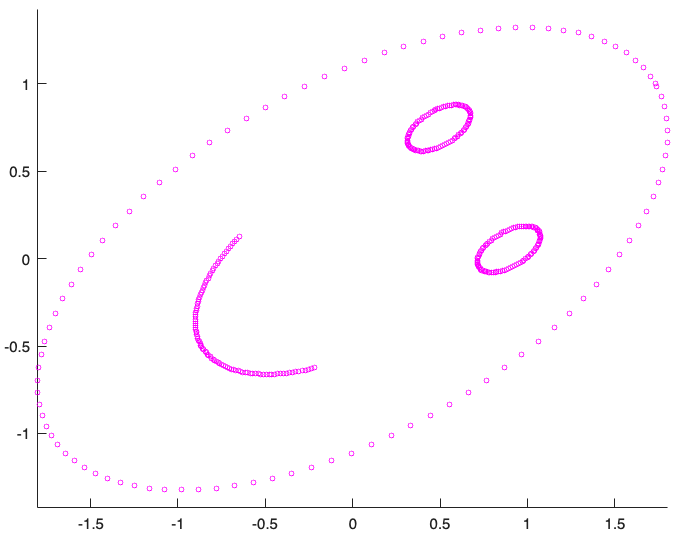
\includegraphics[width=.75\textwidth]{face_stretch_rotate_reflect.png}
        \end{center}

    \end{example}

\end{exploration}

\begin{exploration}\name{Properties of Matrix Multiplication}

    One might expect that, with how much more nuanced matrix multiplication and matrix-vector multiplication are compared to scalar multiplication, that there would be some extra rules and constraints.

    We'll explore these below.

    \begin{example}\name{Allowed mulitplications}

        Whereas we can multiply any scalar by another scalar (unelss we divide by zero), the same is not true for matrices, and also for matrix-vector multiplication.

        The key consideration is that matrices transform vectors in $\R^n$ to vectors in $\R^m$, and so we need to make sure that the matrices are defined to take in $n$-dimensional vectors and output $m$-dimensional vectors.

        Let's use some mapping diagrams to illustrate this for the $3\times 2$ matrix \(M=\begin{bmatrix} 1 & 2 \\ 2&-1 \\ 1 & 1\end{bmatrix}\)

        If $\vec{v}= \begin{bmatrix} 2 \\ 3 \end{bmatrix}$, then $M\vec{v}$ is calculated by $M\vec{v}=2 \begin{bmatrix} 1 \\ 2 \\ 1 \end{bmatrix}+3 \begin{bmatrix} 2 \\ -1 \\ 1 \end{bmatrix}=\begin{bmatrix} 2+6 \\ 4-3 \\ 2+3 \end{bmatrix}=\begin{bmatrix} 8 \\ 1 \\ 5 \end{bmatrix}$.

        Since the columns of $M$ are $3$-dimensional, the result is a $3$-dimensional vector (one for each vector in the linear combination). Since the rows of $M$ are $2$-dimensional, the input vector must be $2$-dimensional (one for each scalar in the linear combination).

        By contrast, if $\vec{v}= \begin{bmatrix} 2 \\ 3 \\ 4 \end{bmatrix}$, then $M\vec{v}$ does not make sense because there isn't a third column of $M$ to multiply by the third entry of $\vec{v}$.

        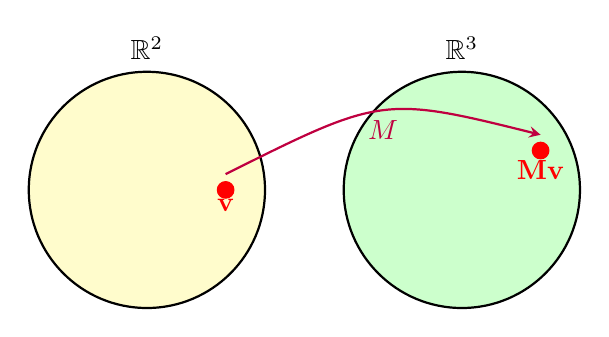
\begin{tikzpicture}

            % Draw sets X, X'
            \draw[fill=yellow!20!white, draw=black, thick] (-4,0) ellipse (1.5cm);
            \draw[fill=green!20!white, draw=black, thick] (0,0) ellipse (1.5cm);
        
            % Labels for sets X, X'
            \node at (-4,1.8) {\(\mathbb{R}^2\)};
            \node at (0,1.8) {\(\mathbb{R}^3\)};
        
            % Elements inside sets
            \filldraw[red] (-3,0) circle (3pt) node[below] {\textbf{v}};
            \filldraw[red] (1,.5) circle (3pt) node[below] {\textbf{Mv}};
        
            % Arrows for the transformation S
            \draw[->, thick, purple] (-3,0.2) .. controls (-1,1.2) .. (1,.7) node[midway, below] {\(M\)};
            
        \end{tikzpicture}

        Detemrine which of the following multiplications make sense, and why.

        $M=\begin{bmatrix} 1 & 2 \\ 2&-1 \\ 1 & 1\end{bmatrix}$, $N=\begin{bmatrix} 1 & 2 & 3 \\ 2&-1 & 0 \\ 1 & 1 & 1\end{bmatrix}$, $P=\begin{bmatrix} 1 & 2 \\ 2&-1 \\ 1 & 1 \\ 0 & 0\end{bmatrix}$

        $v=\begin{bmatrix} 2 \\ 3 \end{bmatrix}$,
        $w=\begin{bmatrix} 2 \\ 3 \\ 4 \end{bmatrix}$, $u=\begin{bmatrix} 2 \\ 3 \\ 4 \\ 5 \end{bmatrix}$

        Select all products that are allowed, make sure that the dimensional description is also correct.

        \begin{selectAll}

            \choice[correct]{$Mv$ is a $3$-dimensional vector}
            \choice{$Mv$ is a $2$-dimensional vector}
            \choice{$Mw$ is a $3$-dimensional vector}
            \choice{$Mw$ is a $2$-dimensional vector}
            \choice{$Mu$ is a $4$-dimensional vector}
            \choice{$Mu$ is a $3$-dimensional vector}
            \choice{$Nv$ is a $3$-dimensional vector}
            \choice{$Nv$ is a $2$-dimensional vector}
            \choice[correct]{$Nw$ is a $3$-dimensional vector}
            \choice{$Nw$ is a $2$-dimensional vector}
            \choice{$Nu$ is a $4$-dimensional vector}
            \choice{$Nu$ is a $3$-dimensional vector}
            \choice[correct]{$Pv$ is a $4$-dimensional vector}
            \choice{$Pv$ is a $3$-dimensional vector}
            \choice{$Pw$ is a $4$-dimensional vector}
            \choice{$Pw$ is a $3$-dimensional vector}
            \choice{$Pu$ is a $4$-dimensional vector}
            \choice{$Pu$ is a $3$-dimensional vector}
        \end{selectAll}

        \begin{solution}

            The matrix $M=\begin{bmatrix} 1 & 2 \\ 2&-1 \\ 1 & 1\end{bmatrix}$ is $3\times 2$, so it can only multiply $2$-dimensional vectors. $Mv$ produces a $3$-dimensional vector from its $3$ rows. 

            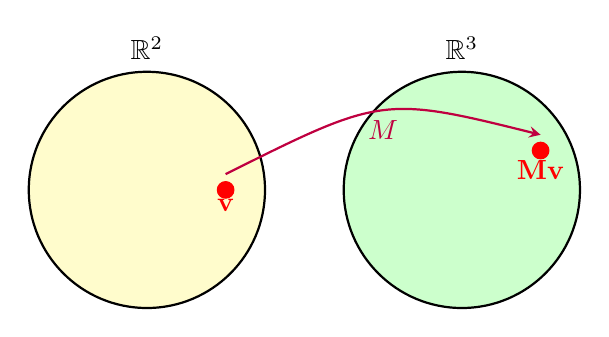
\begin{tikzpicture}

                % Draw sets X, X'
                \draw[fill=yellow!20!white, draw=black, thick] (-4,0) ellipse (1.5cm);
                \draw[fill=green!20!white, draw=black, thick] (0,0) ellipse (1.5cm);
            
                % Labels for sets X, X'
                \node at (-4,1.8) {\(\mathbb{R}^2\)};
                \node at (0,1.8) {\(\mathbb{R}^3\)};
            
                % Elements inside sets
                \filldraw[red] (-3,0) circle (3pt) node[below] {\textbf{v}};
                \filldraw[red] (1,.5) circle (3pt) node[below] {\textbf{Mv}};
            
                % Arrows for the transformation S
                \draw[->, thick, purple] (-3,0.2) .. controls (-1,1.2) .. (1,.7) node[midway, below] {\(M\)};
                
            \end{tikzpicture}

            The matrix $N=\begin{bmatrix} 1 & 2 & 3 \\ 2&-1 & 0 \\ 1 & 1 & 1\end{bmatrix}$ is a $3\times 3$ matrix,
            so it can only multiply $3$-dimensional vectors. $Nw$ produces a $3$-dimensional vector from its $3$ rows.

            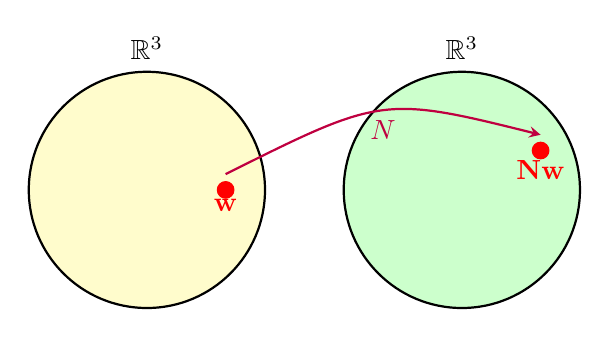
\begin{tikzpicture}

                % Draw sets X, X'
                \draw[fill=yellow!20!white, draw=black, thick] (-4,0) ellipse (1.5cm);
                \draw[fill=green!20!white, draw=black, thick] (0,0) ellipse (1.5cm);
            
                % Labels for sets X, X'
                \node at (-4,1.8) {\(\mathbb{R}^3\)};
                \node at (0,1.8) {\(\mathbb{R}^3\)};
            
                % Elements inside sets
                \filldraw[red] (-3,0) circle (3pt) node[below] {\textbf{w}};
                \filldraw[red] (1,.5) circle (3pt) node[below] {\textbf{Nw}};
            
                % Arrows for the transformation N
                \draw[->, thick, purple] (-3,0.2) .. controls (-1,1.2) .. (1,.7) node[midway, below] {\(N\)};
            
            \end{tikzpicture}

            The matrix $P=\begin{bmatrix} 1 & 2 \\ 2&-1 \\ 1 & 1 \\ 0 & 0\end{bmatrix}$ is $4\times 2$, so it can only multiply $2$-dimensional vectors. $Pv$ produces a $4$-dimensional vector from its $4$ rows.

            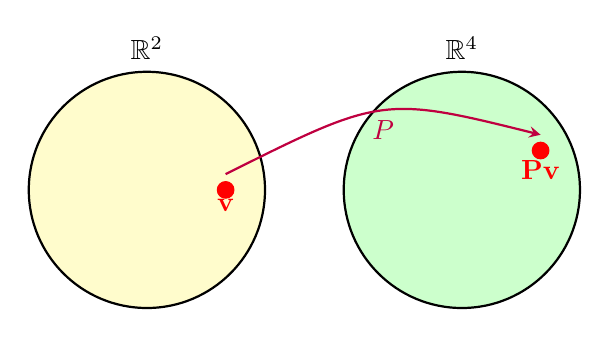
\begin{tikzpicture}

                % Draw sets X, X'
                \draw[fill=yellow!20!white, draw=black, thick] (-4,0) ellipse (1.5cm);
                \draw[fill=green!20!white, draw=black, thick] (0,0) ellipse (1.5cm);
            
                % Labels for sets X, X'
                \node at (-4,1.8) {\(\mathbb{R}^2\)};
                \node at (0,1.8) {\(\mathbb{R}^4\)};
            
                % Elements inside sets
                \filldraw[red] (-3,0) circle (3pt) node[below] {\textbf{v}};
                \filldraw[red] (1,.5) circle (3pt) node[below] {\textbf{Pv}};
            
                % Arrows for the transformation P
                \draw[->, thick, purple] (-3,0.2) .. controls (-1,1.2) .. (1,.7) node[midway, below] {\(P\)};
            
            \end{tikzpicture}

        \end{solution}

        With matrix multiplication, you have to smimilalry consider the dimensions of the vectors after each successive multiplication. You simply need to apply the same reasoning as matrix-vector mulitplication, but keep in mind the dimensions of the output vectors from the first product. If we take the matrices $M$ and $N$ from the previous example, $MN$ would not be allowed because the output of $N$ is $3$-dimensional, and the input of $M$ is $2$-dimensional, so the product would not be defined. 

        $NM$, however, would be allowed because the output of $M$ is $3$-dimensional, and the input of $N$ is $3$-dimensional, so the product would be defined.

        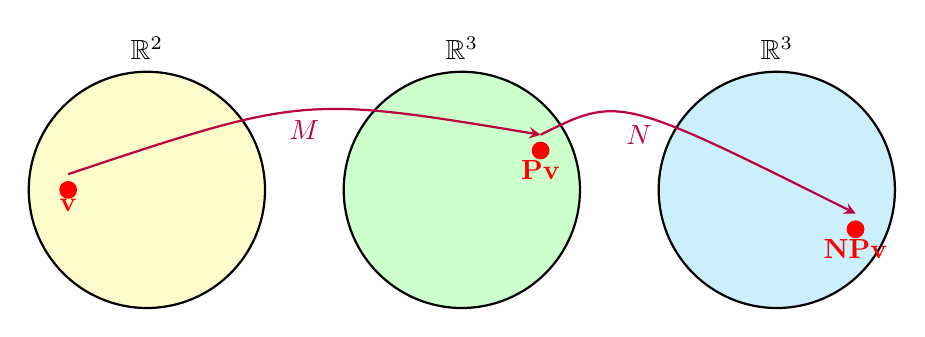
\begin{tikzpicture}

            % Draw sets X, X', and X''
            \draw[fill=yellow!20!white, draw=black, thick] (-4,0) ellipse (1.5cm);  % First ellipse (R^2)
            \draw[fill=green!20!white, draw=black, thick] (0,0) ellipse (1.5cm);    % Second ellipse (R^4)
            \draw[fill=cyan!20!white, draw=black, thick] (4,0) ellipse (1.5cm);     % Third ellipse (R^3)
        
            % Labels for sets X, X', X''
            \node at (-4,1.8) {\(\mathbb{R}^2\)};
            \node at (0,1.8) {\(\mathbb{R}^3\)};
            \node at (4,1.8) {\(\mathbb{R}^3\)};
        
            % Elements inside sets
            \filldraw[red] (-5,0) circle (3pt) node[below] {\textbf{v}};  % Vector in R^2
            \filldraw[red] (1,.5) circle (3pt) node[below] {\textbf{Pv}}; % Vector in R^4
            \filldraw[red] (5,-.5) circle (3pt) node[below] {\textbf{NPv}}; % Vector in R^3
        
            % Arrows for the transformations P and N
            \draw[->, thick, purple] (-5,0.2) .. controls (-2,1.2) .. (1,.7) node[midway, below] {\(M\)};
            \draw[->, thick, purple] (1,.7) .. controls (2,1.2) .. (5,-.3) node[midway, below] {\(N\)};
        
        \end{tikzpicture}

        Now determine which of the following matrix products is allowed, and why, using the matrices %make a 2x3, 3x4, 2x2, 3x3 matrices
        $M=\begin{bmatrix} 1 & 2 & 1\\ 2&-1 &0\end{bmatrix}$, $N=\begin{bmatrix} 1 & 2 & 3 \\ 2&-1 & 0 \\ 1 & 1 & 1 \\ 0 & 0 & 0\end{bmatrix}$, $P=\begin{bmatrix} 1 & 2 \\ 2&-1 \end{bmatrix}$, $Q=\begin{bmatrix} 1 & 2 & 3 \\ 2&-1 & 0 \\ 1 & 1 & 1\end{bmatrix}$.


        \begin{selectAll}

            \choice{$MN$}
            \choice[correct]{$MN^T$}
            \choice{$NM$}
            \choice{$NM^T$}
            \choice{$MP$}
            \choice[correct]{$M^TP$}
            \choice{$PQ$}
            \choice{$QP$}
            \choice{$PQ^T$}
            \choice[correct]{$NQ$}
            \choice{$N^TQ$}
            \choice[correct]{$PM$}

        \end{selectAll}

        \begin{solution}
        
            $N^T$ is a $3\times 4$ matrix, so it outputs a $3$-dimensional vector. $M$ is a $2\times 3$ matrix, so it takes in a $3$-dimensional vector and thus the product $MN^T$ is allowed.

            $P$ is a $2\times 2$ matrix, so it outputs a $2$-dimensional vector. $M^T$ is a $3\times 2$ matrix, so it takes in a $2$-dimensional vector and thus the product $M^TP$ is allowed.

            $Q$ is a $3\times 3$ matrix, so it outputs a $3$-dimensional vector. $N$ is a $4\times 3$ matrix, so it takes in a $3$-dimensional vector and thus the product $NQ$ is allowed.

            $M$ is a $2\times 3$ matrix, so it outputs a $2$-dimensional vector. $P$ is a $2\times 2$ matrix, so it takes in a $2$-dimensional vector and thus the product $PM$ is allowed.

        \end{solution}

    \end{example}

    \begin{example}\name{Commutativity}

        Scalar multiplication is commutative, meaning you can swap the order of any numbers in the product and still get the same result.

        For instance, $3\cdot 4\cdot 5\cdot 2=2\cdot 5\cdot 4\cdot 3=4\cdot 3\cdot 5\cdot 2=120$.

        Let's check whether we can do the same for matrix multiplication. In our past example, we got the composite matrix $M=FRS$, a stretch by $2$, a $60^\circ$ rotation, and a reflection about the $y$-axis.

        If matrix multiplication is commutative, then the matrices $FSR$ and $RFS$ should give us the same result as $M$, since it wouldn't matter what order we multiplied the matrices in.

        Do this in MATLAB and match the results of each product.

        \begin{hint}

            You can use the same code as before, but just change the order of the matrices in the product. Match each figure to the matrices that produced them.

        \end{hint}

        % Include the FSR image
        \begin{figure}[ht!]
            \centering
            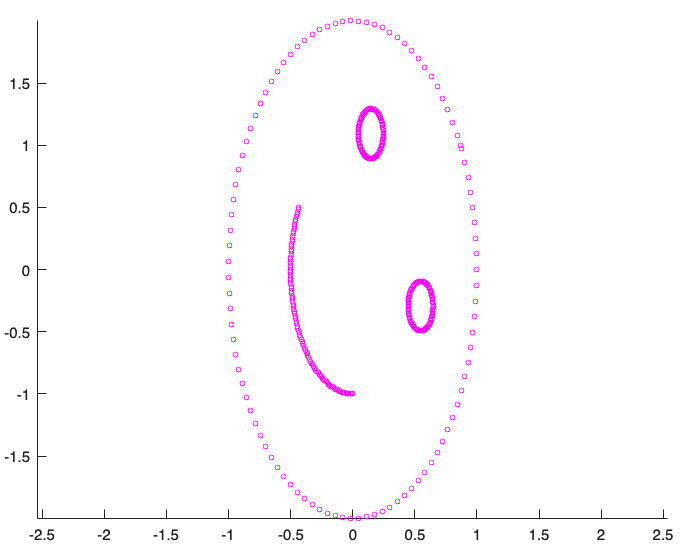
\includegraphics[width=.5\textwidth]{fsr.png}
            \caption{(a)}
        \end{figure}
        
        \begin{selectAll}

            \choice[correct]{$FSR$}
            \choice{$RSF$}
            \choice[correct]{$SFR$}
            \choice{$SRF$}

        \end{selectAll}

        % Include the SRF image
        \begin{figure}[ht!]
            \centering
            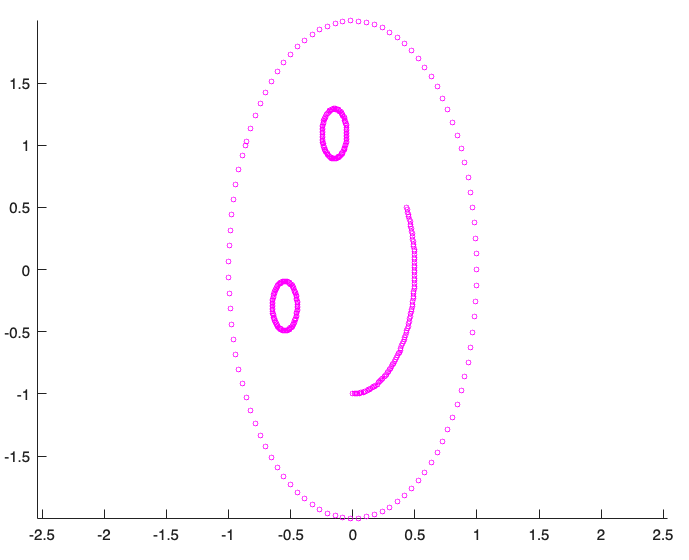
\includegraphics[width=.5\textwidth]{srf.png}
            \caption{(c)}
        \end{figure}

        \begin{selectAll}

            \choice{$FSR$}
            \choice{$RSF$}
            \choice{$SFR$}
            \choice[correct]{$SRF$}           

        \end{selectAll}

        % Include the RSF image
        \begin{figure}[ht!]
            \centering
            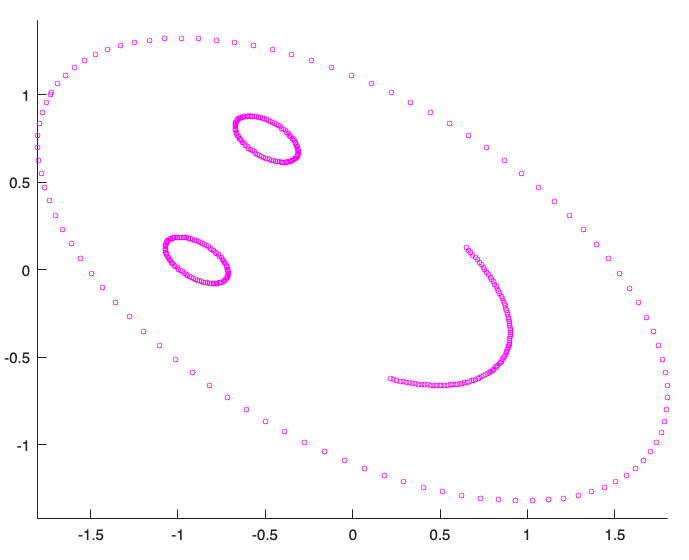
\includegraphics[width=.5\textwidth]{rsf.png}
            \caption{(d)}
        \end{figure}

        \begin{selectAll}

            \choice{$FSR$}
            \choice[correct]{$RSF$}
            \choice{$SFR$}
            \choice{$SRF$}

        \end{selectAll}

    As we can see, while there is some overlap, different orders of matrix multiplication produced different transformations of the inptu vectors in $\R^2$. We have to conclude that the ordering matters for matrix multiplication, and so \emph{matrix multiplication is not commutative}.

    \end{example}

    \begin{example}\name{Associativity}

        Associativity regards the order in which each pair of operations is carried out. For instance, $(3\cdot 4)\cdot 5=12\cdot 5=60$, and $3\cdot (4\cdot 5)=3\cdot 20=60$, so even though we carried out each multiplication in a different order, we still got the same result.

        Is this also true for matrices? Let's check.

        Use the following code, which computes each pair of matrices before the for loop, and then apply the pairs in different orders to check for associativity.

        First, compute $F(RS)$.

        \vspace{1cm}


$\texttt{load +linalg/face\_points.mat}$

$\texttt{R = [cosd(60) -sind(60); sind(60) cosd(60)]}$

$\texttt{S = [1 0; 0 2]}$

$\texttt{F = [-1 0; 0 1]}$

$\texttt{RS = }\answer[given,format=string]{R}*\answer[format=string]{S}$

$\texttt{FR = }\answer[given,format=string]{F}*\answer[format=string]{R}$

$\texttt{for i=1:length(face\_points)}$

$\qquad \texttt{face\_points(i,:) = }\answer[given,format=string]{RS}\texttt{*face\_points(i,:)';}$

$\qquad \texttt{face\_points(i,:) = }\answer[format=string]{F}\texttt{*face\_points(i,:)';}$

$\texttt{end}$

$\texttt{linalg.plot\_img\_points(face\_points)}$

\vspace{1cm}

        Then, compute $(FR)S$.

        \vspace{1cm}

$\texttt{for i=1:length(face\_points)}$

$\qquad \texttt{face\_points(i,:) = }\answer[given,format=string]{S}\texttt{*face\_points(i,:)';}$

$\qquad \texttt{face\_points(i,:) = }\answer[format=string]{FR}\texttt{*face\_points(i,:)';}$

$\texttt{end}$

$\texttt{linalg.plot\_img\_points(face\_points)}$

\vspace{1cm}

These should all give you the same smiley face that we originally stretched, rotated, and reflected.

So, matrix multiplicaiton \emph{is associative}.

    \end{example}

\end{exploration}

\begin{remark}

    As we continue to learn more properties of matrices, and which matrices are useful for solving various problems, remember that most (if not all) of the powerful things that we can do with matrices boil down to the understanding of matrices as linear transformations.

\end{remark}

\end{document}